\documentclass{beamer} \useoutertheme{infolines}
\usefonttheme{default}

\usepackage{xcolor}     % for defining colors
\usepackage{multicol}   % for multiple columns
\usepackage{etoolbox}   % for toggles
\usepackage{subcaption} % for subplots
\usepackage{listings}   % for colored verbatim
\usepackage{listings}   % for colored verbatim
\usepackage{ifthen}     % for conditionals
% required packages
\usepackage{xcolor}
\usepackage{stmaryrd} % jump brackets: \llbracket, \rrbracket

% create a provideenvironment command
\makeatletter
\def\provideenvironment{\@star@or@long\provide@environment}
\def\provide@environment#1{%
  \@ifundefined{#1}%
    {\def\reserved@a{\newenvironment{#1}}}%
    {\def\reserved@a{\renewenvironment{dummy@environ}}}%
  \reserved@a
}
\def\dummy@environ{}
\makeatother

% directories
\newcommand{\diagramdirectory}{../diagrams}

% general
\newcommand{\x}{\mathbf{x}}
\newcommand{\qpoint}{\x_q}
\newcommand{\timevalue}{t}
\newcommand{\timestepsize}{\Delta\timevalue}
\newcommand{\dt}{\timestepsize}
\newcommand{\timeindex}{n}
\newcommand{\speed}{v}
\newcommand{\velocity}{\mathbf{\speed}}
\newcommand{\velocityx}{u}
\newcommand{\velocityy}{v}
\newcommand{\velocityn}{v_n}
\newcommand{\vx}{\velocityx}
\newcommand{\vy}{\velocityy}
\newcommand{\vn}{\velocityn}

% normal vector
\newcommand{\normalvectorletter}{n}
\newcommand{\normalvector}{\mathbf{\normalvectorletter}}
\newcommand{\normalx}{\normalvectorletter_x}
\newcommand{\normaly}{\normalvectorletter_y}
\newcommand{\nx}{\normalx}
\newcommand{\ny}{\normaly}

\newcommand{\ndimensions}{N_\text{dim}}
\newcommand{\ncomponents}{m}
\newcommand{\ndofs}{N_\text{dof}}
\newcommand{\nnodes}{N_\text{node}}
\newcommand{\dofindex}{j}
\newcommand{\nodeindex}{k}
\newcommand{\componentindex}{k}
\newcommand{\transpose}{^{\text{T}}}

% schemes
\newcommand{\low}{L}
\newcommand{\high}{H}

% solution
\newcommand{\scalarsolution}{u}
\newcommand{\vectorsolution}{\mathbf{\scalarsolution}}
\newcommand{\approximate}[1]{\tilde{#1}}
\newcommand{\approximatescalarsolution}{\approximate{\scalarsolution}}
\newcommand{\approximatevectorsolution}{\approximate{\vectorsolution}}
\newcommand{\solutionletter}{U}
\newcommand{\solutionvector}{\mathbf{\solutionletter}}
\newcommand{\U}{\solutionvector}
\newcommand{\lowordersolution}[1][]{
  \ifthenelse{\equal{#1}{}}{\solutionvector^L}{\solutionvector^{L,#1}}}
\newcommand{\highordersolution}[1][]{
  \ifthenelse{\equal{#1}{}}{\solutionvector^H}{\solutionvector^{H,#1}}}

% math
\newcommand{\triangulation}{\mathcal{K}_h}
\newcommand{\approximationspace}{\mathcal{U}_h}
\newcommand{\approximationspaceinc}{\approximationspace^{\textup{inc}}}
\newcommand{\referenceelementmap}{\Phi}
\newcommand{\qonespace}{\mathbb{Q}_1}

% sets
\newcommand{\faces}{\mathcal{F}}
\newcommand{\quadraturepoints}{\mathcal{Q}}

% domain and FEM
\newcommand{\domain}{\mathcal{D}}
\newcommand{\celldomain}[1][\cell]{\domain_#1}
\newcommand{\facedomain}{\domain}
\newcommand{\domainboundary}{\partial\domain}
\newcommand{\incomingdomainboundary}{\domainboundary^{\textup{inc}}}
\newcommand{\cellindex}{K}
\newcommand{\cell}{K}
\newcommand{\celldiameter}{\Delta x}
\newcommand{\maxcelldiameter}{\Delta x_{\text{max}}}
\newcommand{\volume}{V}
\newcommand{\dvolume}{\,d\x}
\newcommand{\area}{A}
\newcommand{\darea}{\,d\area}
\newcommand{\testfunction}{\varphi}
\newcommand{\vectortestfunctionscalar}{\Phi}
\newcommand{\vectortestfunction}{\mathbf{\vectortestfunctionscalar}}
\newcommand{\support}{S}
\newcommand{\maxdof}{N}
\newcommand{\interpolant}{\Pi}

% local viscous bilinear form
\newcommand{\localvisc}{b}
\newcommand{\localviscbilinearform}[3]{\localvisc_#1(\testfunction_#2, \testfunction_#3)}
\newcommand{\cellvolume}{|\celldomain|}
\newcommand{\cardinality}[1][]{\ifthenelse{\equal{#1}{}}{n_\cell}{n_#1}}
\newcommand{\cardsystem}{\bar{n}}
\newcommand{\indices}{\mathcal{I}}
\newcommand{\cellindices}{\mathcal{K}}
\newcommand{\indicesnode}{\indices^{\text{node}}_\cell}
\newcommand{\indicescell}[1][]{\ifthenelse{\equal{#1}{}}{\indices_\cell}
  {\indices_{#1}}}
\newcommand{\incomingindices}{\indices^{\textup{inc}}}
\newcommand{\notincomingindices}{\indices(\triangulation)\setminus\incomingindices}

% entropy viscosity
\newcommand{\entropy}{\eta}
\newcommand{\entropyflux}{\mathbf{\consfluxletter}^\eta}
\newcommand{\entropyjump}{\mathcal{J}}
\newcommand{\entropyresidual}{\mathcal{R}}
\newcommand{\entropyresidualcoef}{c_\entropyresidual}
\newcommand{\entropyjumpcoef}{c_\entropyjump}
\newcommand{\entropynormalization}{\hat{\entropy}}

% conservation law
\newcommand{\consfluxletter}{f}
\newcommand{\consflux}{\mathbf{\consfluxletter}}
\newcommand{\consfluxsystem}{\mathbf{\MakeUppercase{\consfluxletter}}}
\newcommand{\consfluxscalar}[1][\scalarsolution]{\mathbf{\consfluxletter}(#1)}
\newcommand{\consfluxvector}{\mathbf{\MakeUppercase{\consfluxletter}}}
\newcommand{\consfluxvectory}{\mathbf{G}}
\newcommand{\consfluxvectorn}{\consfluxvector_{n}}
\newcommand{\consfluxinterpolant}{\mathrm{F}}
\newcommand{\conssource}{\mathbf{s}}

% viscosity
\newcommand{\viscosity}{\nu}
\newcommand{\cellviscosity}{\viscosity_\cellindex}
\newcommand{\lowordercellviscosity}[1][]{
  \ifthenelse{\equal{#1}{}}{\cellviscosity^L}
  {\cellviscosity^{L,#1}}}
\newcommand{\highordercellviscosity}[1][]{
  \ifthenelse{\equal{#1}{}}{\cellviscosity^H}
  {\cellviscosity^{H,#1}}}
\newcommand{\entropycellviscosity}[1][]{
  \ifthenelse{\equal{#1}{}}{\cellviscosity^\entropy}
  {\cellviscosity^{\entropy,#1}}}

% viscous fluxes
\newcommand{\viscstring}{\text{visc}}
\newcommand{\viscflux}[1]{\mathbf{\consfluxletter}^{\viscstring,#1}}
\newcommand{\viscconsfluxvector}
  {\mathbf{\MakeUppercase{\consfluxletter}}^\viscstring
  (\vectorsolution,\viscosity)}

% mass matrix
\newcommand{\massmatrixletter}{M}
\newcommand{\massmatrix}{\mathbf{\massmatrixletter}}
\newcommand{\M}{\massmatrix}
\newcommand{\consistentmassmatrix}{\massmatrix^C}
\newcommand{\consistentmassentry}{\massmatrixletter^C_{i,j}}
\newcommand{\lumpedmassmatrix}{\massmatrix^L}
\newcommand{\lumpedmassentry}{\massmatrixletter^L_{i,i}}

% gradient matrix (for conservation law systems)
\newcommand{\gradientmatrixletter}{c}
\newcommand{\gradientmatrix}{\mathbf{\MakeUppercase{\gradientmatrixletter}}}
\newcommand{\gradiententry}{\mathbf{\gradientmatrixletter}\ij}

% steady-state system matrix and rhs
\newcommand{\ssmatrixletter}{A}
\newcommand{\ssmatrix}[1][]{
  \ifthenelse{\equal{#1}{}}
  {\mathbf{\ssmatrixletter}}
  {\mathbf{\ssmatrixletter}^#1}}
\newcommand{\A}{\ssmatrix}
\newcommand{\loworderssmatrix}[1][]{
  \ifthenelse{\equal{#1}{}}
  {\ssmatrix^L}
  {\ssmatrix^{L,#1}}}
\newcommand{\highorderssmatrix}[1][]{
  \ifthenelse{\equal{#1}{}}
  {\ssmatrix^H}
  {\ssmatrix^{H,#1}}}
\newcommand{\ssrhsletter}{b}
\newcommand{\ssrhs}[1][]{
  \ifthenelse{\equal{#1}{}}
  {\mathbf{\ssrhsletter}}
  {\mathbf{\ssrhsletter}^#1}}
\renewcommand{\b}{\ssrhs}
\newcommand{\ssresletter}{r}
\newcommand{\ssres}{\mathbf{\ssresletter}}
\renewcommand{\r}{\ssres}
\newcommand{\B}{\mathbf{B}}
\newcommand{\s}{\mathbf{s}}

% diffusion matrix
\newcommand{\diffusionmatrixletter}{D}
\newcommand{\diffusionmatrix}[1][]{
  \ifthenelse{\equal{#1}{}}
  {\mathbf{\diffusionmatrixletter}}
  {\mathbf{\diffusionmatrixletter}^#1}}
\newcommand{\D}{\diffusionmatrix}
\newcommand{\loworderdiffusionmatrix}[1][]{
  \ifthenelse{\equal{#1}{}}
  {\diffusionmatrix^L}
  {\diffusionmatrix^{L,#1}}}
\newcommand{\highorderdiffusionmatrix}[1][]{
  \ifthenelse{\equal{#1}{}}
  {\diffusionmatrix^H}
  {\diffusionmatrix^{H,#1}}}

% Runge-Kutta
\newcommand{\RKstagesolution}{\hat{\mathbf{\solutionletter}}}
\newcommand{\RKintermediatesolution}{\tilde{\mathbf{\solutionletter}}}
\newcommand{\RKoldsolutioncoef}{\alpha}
\newcommand{\RKstagesolutioncoef}{\beta}
\newcommand{\RKtimecoef}{c}
\newcommand{\RKstagetime}{\hat{\timevalue}}
\newcommand{\RKnstages}{s}

% FCT
\newcommand{\solutionbound}{W}
\newcommand{\DMPlowerbound}{\solutionbound^{\textup{DMP},-}}
\newcommand{\DMPupperbound}{\solutionbound^{\textup{DMP},+}}
\newcommand{\DMPlowerboundss}{\solutionbound^{\textup{DMP},\textup{ss},-}}
\newcommand{\DMPupperboundss}{\solutionbound^{\textup{DMP},\textup{ss},+}}
\newcommand{\DMPboundsss}{\solutionbound^{\textup{DMP},\textup{ss},\pm}}
\newcommand{\DMPlowerboundee}{\solutionbound^{\textup{DMP},\textup{ee},-}}
\newcommand{\DMPupperboundee}{\solutionbound^{\textup{DMP},\textup{ee},+}}
\newcommand{\DMPboundsee}{\solutionbound^{\textup{DMP},\textup{ee},\pm}}
\newcommand{\DMPlowerboundtheta}{\solutionbound^{\textup{DMP},\textup{theta},-}}
\newcommand{\DMPupperboundtheta}{\solutionbound^{\textup{DMP},\textup{theta},+}}
\newcommand{\DMPboundstheta}{\solutionbound^{\textup{DMP},\textup{theta},\pm}}
\newcommand{\DMPbounds}{\solutionbound^{\textup{DMP},\pm}}
\newcommand{\analyticDMPbounds}{\solutionbound^{\textup{analytic},\pm}}
\newcommand{\analyticDMPupperbound}{\solutionbound^{\textup{analytic},+}}
\newcommand{\analyticDMPlowerbound}{\solutionbound^{\textup{analytic},-}}
\newcommand{\limitedfluxbound}{Q}
\newcommand{\antidiffusionbound}{\limitedfluxbound}
\newcommand{\antidiffusionboundvector}{\mathbf{\limitedfluxbound}}
\newcommand{\antidiffusionlowerboundss}{\antidiffusionbound^{\textup{ss},-}}
\newcommand{\antidiffusionupperboundss}{\antidiffusionbound^{\textup{ss},+}}
\newcommand{\antidiffusionlowerboundee}{\antidiffusionbound^{\textup{ee},-}}
\newcommand{\antidiffusionupperboundee}{\antidiffusionbound^{\textup{ee},+}}
\newcommand{\antidiffusionlowerboundtheta}{\antidiffusionbound^{\textup{theta},-}}
\newcommand{\antidiffusionupperboundtheta}{\antidiffusionbound^{\textup{theta},+}}
\newcommand{\limitedfluxboundsi}{\limitedfluxbound^\pm_i}
\newcommand{\limiterletter}{L}
\newcommand{\limitermatrix}{\mathbf{\limiterletter}}
\newcommand{\correctionfluxletter}{p}
\newcommand{\correctionfluxvector}{\mathbf{\correctionfluxletter}}
\newcommand{\correctionfluxentry}{\MakeUppercase{\correctionfluxletter}}
\newcommand{\correctionfluxij}{\correctionfluxentry_{i,j}}
\newcommand{\correctionfluxji}{\correctionfluxentry_{j,i}}
\newcommand{\correctionfluxmatrix}{\mathbf{\MakeUppercase{\correctionfluxletter}}}
\newcommand{\antidiffusiveflux}{\correctionfluxentry}

% remainder
\newcommand{\correctionfluxremainder}{\Delta\MakeUppercase{\correctionfluxletter}}
\newcommand{\correctionfluxmatrixremainder}{\Delta\correctionfluxmatrix}
\newcommand{\limitedcorrectionfluxmatrixremainder}
  {\bar{\correctionfluxmatrixremainder}}

\newcommand{\limitedcorrectionfluxletter}{\bar{\correctionfluxletter}}
\newcommand{\cumulativecorrectionfluxletter}{\bar{\correctionfluxletter}}
\newcommand{\cumulativecorrectionfluxvector}{\bar{\correctionfluxvector}}
\newcommand{\cumulativecorrectionfluxvectorchange}
  {\Delta\cumulativecorrectionfluxvector}
\newcommand{\correctionfluxsumsi}{\MakeUppercase{\correctionfluxletter}^\pm_i}
\newcommand{\limitedfluxsum}{\limitermatrix\cdot\correctionfluxmatrix}
\newcommand{\limitedfluxsumi}{\sumj\limiterletter\ij
  \MakeUppercase{\correctionfluxletter}\ij}
\newcommand{\F}{\correctionfluxmatrix}
\newcommand{\LF}{\limitermatrix\cdot\correctionfluxmatrix}
\newcommand{\transformationmatrix}{\mathbf{T}}

% radiation transport
\newcommand{\angularflux}{\psi}
\newcommand{\scalarflux}{\phi}
\newcommand{\speedoflight}{c}
\newcommand{\totalcrosssection}{\Sigma_\text{t}}
\newcommand{\reactioncoef}{\sigma}
\newcommand{\directionvector}{\mathbf{\Omega}}
\newcommand{\di}{\directionvector}
\newcommand{\xdet}{(\x,\di,E,t)}
\newcommand{\xet}{(\x,E,t)}
\newcommand{\scalarsource}{q}
\newcommand{\radiationsource}{Q}

% Euler equations
\newcommand{\density}{\rho}
\newcommand{\totalenergy}{E}
\newcommand{\momentum}{\mathbf{m}}
\newcommand{\pressure}{p}
\newcommand{\gasconstant}{\gamma}
\newcommand{\identity}{\mathbf{I}}

% shallow water equations
\newcommand{\height}{h}
\newcommand{\heightmomentumletter}{q}
\newcommand{\heightmomentum}{\mathbf{\heightmomentumletter}}
\newcommand{\heightmomentumx}{\heightmomentumletter_x}
\newcommand{\heightmomentumy}{\heightmomentumletter_y}
\newcommand{\heightmomentumd}{\heightmomentumletter_d}
\newcommand{\dischargex}{\heightmomentumletter}
\newcommand{\bathymetry}{b}
\newcommand{\waterlevel}{w}
\newcommand{\gravity}{g}
\newcommand{\speedofsound}{a}
\newcommand{\froude}{\mathrm{Fr}}

% Riemann solvers
\newcommand{\shockspeed}{S}
\newcommand{\eigenvalue}{\lambda}
\newcommand{\eigenvaluematrix}{\mathbf{\Lambda}}
\newcommand{\eigenvector}{\mathbf{k}}
\newcommand{\eigenvectormatrix}{\mathbf{K}}
\newcommand{\jacobianx}{\mathbf{A}}
\newcommand{\jacobiany}{\mathbf{B}}
\newcommand{\jacobiann}{\jacobianx_{n}}
\newcommand{\characteristicsolution}{\mathbf{w}}
\newcommand{\wavespeed}{\eigenvalue}
\newcommand{\maxwavespeed}[1][]{
  \ifthenelse{\equal{#1}{}}{\wavespeed^{\text{max}}}{\wavespeed^{\text{max},#1}}}
\newcommand{\wavestrength}{\mathcal{W}}

%==============================================================================
% colors
\colorlet{lightBlue}{blue!20!white}
\colorlet{lightGreen}{green!20!white}

% indexing
\renewcommand{\ij}{_{i,j}}
\newcommand{\ji}{_{j,i}}
\newcommand{\kl}{_{k,\ell}}
\newcommand{\lk}{_{\ell,k}}
\newcommand{\nodei}{_{\nodeindex(i)}}
\newcommand{\nodej}{_{\nodeindex(j)}}
\newcommand{\nodeij}{_{\nodeindex(i),\nodeindex(j)}}
\newcommand{\nodeji}{_{\nodeindex(j),\nodeindex(i)}}
\newcommand{\nodequantity}[1]{\underline{#1}}

% sums and integrals
\newcommand{\sumj}{\sum\limits_j}
\newcommand{\sumjnoti}{\sum\limits_{j\ne i}}
\newcommand{\sumKSi}{\sum\limits_{\cell\in\cellindices(\support_i)}}
%\newcommand{\sumKSij}[1][\cell]
%  {\sum\limits_{#1:\celldomain[#1]\subset\support_{i,j}}}
\newcommand{\sumKSij}[1][\cell]
  {\sum\limits_{#1\in\cellindices(\support\ij)}}
\newcommand{\sumallcells}{\sum\limits_{\cell}}
\newcommand{\intdomain}[1]{\int\limits_\domain #1 \,\dvolume}
\newcommand{\intboundary}[1]{\int\limits_{\domainboundary} #1 \,d\area}
\newcommand{\intSi}{\int\limits_{\support_i}}
\newcommand{\intSij}{\int\limits_{\support_{i,j}}}

% math
\newcommand{\ltwonorm}[1]{\left\|#1\right\|_{L^2}} % L-2 norm

% BC
\newcommand{\interior}{^{\text{in}}}
\newcommand{\BC}{^{\text{BC}}}

% common fractions
\newcommand{\half}{\frac{1}{2}}
\newcommand{\fourth}{\frac{1}{4}}

% derivatives
\newcommand{\dd}[2]{\frac{d #1}{d #2}}               % ordinary derivative
\newcommand{\pd}[2]{\frac{\partial #1}{\partial #2}} % partial derivative
\newcommand{\ppt}[1]{\pd{#1}{t}}                     % partial d/dt
\newcommand{\ppx}[1]{\pd{#1}{x}}                     % partial d/dx
\newcommand{\ppy}[1]{\pd{#1}{y}}                     % partial d/dy
\newcommand{\ddt}[1]{\frac{d#1}{dt}}                 % ordinary d/dt

% typesetting
\newcommand{\pr}[1]{\left(#1\right)} % parentheses
\newcommand{\sq}[1]{\left[#1\right]} % square brackets
\newcommand{\jumpbrackets}[1]{\left\llbracket#1\right\rrbracket} % jump brackets
\newcommand{\tab}{\hspace*{0.5cm}}   % tab for verbatim evironments
\newcommand{\eqp}{\,.} % equation period
\newcommand{\eqc}{\,,} % equation comma

% miscellaneous
\newcommand{\xt}{\pr{\x,\timevalue}}
\newcommand{\divergence}{\nabla\cdot}
\newcommand{\unitvector}[1]{\hat{\mathbf{e}}_{#1}}

% command to highlight term in equation
\newcommand{\highlightblue}[1]{
  \colorbox{lightBlue}{$\displaystyle#1$}}
\newcommand{\highlightgreen}[1]{
  \colorbox{lightGreen}{$\displaystyle#1$}}

% QED symbol command
\providecommand{\qed}{\nobreak \ifvmode \relax \else
  \ifdim\lastskip<1.5em \hskip-\lastskip
  \hskip1.5em plus0em minus0.5em \fi \nobreak
  \vrule height0.75em width0.5em depth0.25em\fi}

% math environments
\provideenvironment{proof}[1][Proof]{\begin{trivlist}
\item[\hskip \labelsep {\bfseries #1}]}{\end{trivlist}}
\provideenvironment{example}[1][Example]{\begin{trivlist}
\item[\hskip \labelsep {\bfseries #1}]}{\end{trivlist}}
\newenvironment{remark}[1][Remark]{\begin{trivlist}
\item[\hskip \labelsep {\bfseries #1}]}{\end{trivlist}}

% table environment
% #1 = caption
% #2 = label
% #3 = table format (columns)
% #4 = header row
\newenvironment{mytable}[4]
  {\begin{table}[htb]\caption{#1\label{tab:#2}}\begin{center}
    \begin{tabular}
    {#3}\hline #4\\\hline}
  {\hline\end{tabular}\end{center}\end{table}}

% references commands
%\newcommand{\refsec}[1]{, \S#1}
\newcommand{\refsec}[1]{}

% algorithm shortcuts
\newcommand{\objective}{\phi}
\newcommand{\hmin}{\height_{\text{min}}}
\newcommand{\hmax}{\height_{\text{max}}}
\newcommand{\hlow}{\check{\height}}
\newcommand{\hhigh}{\hat{\height}}
\newcommand{\hrarefaction}{\tilde{\height}_*}
\newcommand{\tol}{\epsilon}
\newcommand{\minwavespeed}{\wavespeed_{\text{min}}}
\newcommand{\lowwavespeedone}{\check{\wavespeed}_1}
\newcommand{\highwavespeedone}{\hat{\wavespeed}_1}
\newcommand{\lowwavespeedtwo}{\check{\wavespeed}_2}
\newcommand{\highwavespeedtwo}{\hat{\wavespeed}_2}
\newcommand{\hinterplow}{\height_d}
\newcommand{\hinterphigh}{\height_u}

% checkboxes
\usepackage{amssymb}
\usepackage{xcolor}
\definecolor{myorangeheavy}{RGB}{255,150,0}
\newcommand{\checked}{
  \makebox[0pt][l]{$\square$}\raisebox{.15ex}
  {\hspace{0.1em}\textcolor{myorangeheavy}{$\checkmark$}}}
\newcommand{\unchecked}{
  \makebox[0pt][l]{$\square$}\hspace{0.9em}}

% highlighting
\newcommand{\hlorange}[1]{\textcolor{myorangeheavy}{#1}}

% invariant domains
\newcommand{\invariantset}{A}
\newcommand{\admissibleset}{\mathcal{A}}
\newcommand{\discreteprocess}{R}
\newcommand{\convexcoefficient}{a}
\newcommand{\convexelement}{\mathbf{b}}

% spaces
\newcommand{\realspace}[1][]{
  \ifthenelse{\equal{#1}{}}{\mathbb{R}}{\mathbb{R}^{#1}}}

% nonlinear solve
\newcommand{\nonlinearmatrix}{\mathbf{B}}
\newcommand{\nonlinearrhs}{\mathbf{s}}
\newcommand{\relaxationparameter}{\alpha}
\newcommand{\nonlineartolerance}{\epsilon}

% algorithm
\usepackage{algpseudocode}
\usepackage{algorithm}
\newcommand{\Break}{\State \textbf{break}}
\newcommand{\Not}{\textbf{not}\,}
\newcommand{\Error}[1]{\State \textbf{error}: #1}

% boundary conditions
\newcommand{\dirichlet}[1]{\tilde{#1}}

\newcommand{\rowsum}[1]{#1\mathbf{1}}

% convergence and error analysis
\newcommand{\order}{\mathcal{O}}
\newcommand{\err}{e}
\newcommand{\dx}{\Delta x}

% tolerance adjustment for line-breaking, to prevent \overfull warnings
\newenvironment{tolerant}[1]{
  \par\tolerance=#1\relax
}{
  \par
}
 % macros file

% create toggle for print-friendly mode (no colored heading and sidebar)
\newtoggle{PRINTMODE}
\togglefalse{PRINTMODE} %\toggletrue or \togglefalse

% add sidebar if not in print mode
\setbeamertemplate{items}[square]
\setbeamertemplate{navigation symbols}{}

% define colors
\definecolor{myblue}{RGB}{60,140,230}
\definecolor{myorangelight}{RGB}{255,220,0}
\definecolor{myorangemedium}{RGB}{255,190,50}
\definecolor{myorangeheavy}{RGB}{255,150,0}
\definecolor{myorangered}{RGB}{255,100,30}
\definecolor{mygray}{RGB}{100,100,100}

\colorlet{primarycolor}{myblue}
\colorlet{secondarycolorlight}{myorangelight}
\colorlet{secondarycolormedium}{myorangemedium}
\colorlet{secondarycolorheavy}{myorangeheavy}
\colorlet{secondarytextcolor}{myorangered}

% make headers black on white if in print mode, colored otherwise
\iftoggle{PRINTMODE}{
   \setbeamercolor{title}{fg=black,bg=white}
   \setbeamercolor{frametitle}{fg=black,bg=white}
}{
   \setbeamercolor{title}{fg=primarycolor,bg=white}
   \setbeamercolor{frametitle}{fg=white,bg=primarycolor}
}

% colors
\setbeamercolor{normal text}{fg=mygray}
\setbeamercolor{item projected}{fg=white,bg=secondarycolorheavy}
\setbeamercolor{itemize item}{fg=secondarycolorheavy}
\setbeamercolor{itemize subitem}{fg=secondarycolormedium}
\setbeamercolor{itemize subsubitem}{fg=secondarycolorlight}
%\setbeamercolor{author in head/foot}{fg=secondarytextcolor,bg=secondarycolorlight}
%\setbeamercolor{title in head/foot}{fg=secondarytextcolor,bg=secondarycolormedium}
%\setbeamercolor{date in head/foot}{fg=white,bg=secondarycolorheavy}
\setbeamercolor{author in head/foot}{fg=white,bg=secondarycolormedium}
\setbeamercolor{title in head/foot}{fg=white,bg=secondarycolormedium}
\setbeamercolor{date in head/foot}{fg=white,bg=secondarycolormedium}

% no header
\setbeamertemplate{headline}{}

% custom footer
\makeatletter
\setbeamertemplate{footline}
{
  \leavevmode%
  \hbox{%
  \begin{beamercolorbox}[wd=.333333\paperwidth,ht=2.25ex,dp=1ex,center]{author in head/foot}%
    \usebeamerfont{author in head/foot}\insertsection
  \end{beamercolorbox}%
  \begin{beamercolorbox}[wd=.333333\paperwidth,ht=2.25ex,dp=1ex,center]{title in head/foot}%
    \usebeamerfont{title in head/foot}\insertsubsection
  \end{beamercolorbox}%
  \begin{beamercolorbox}[wd=.333333\paperwidth,ht=2.25ex,dp=1ex,right]{date in head/foot}%
    \usebeamerfont{date in head/foot}\insertshortdate{}\hspace*{2em}
    \insertframenumber{} / \inserttotalframenumber\hspace*{2ex} 
  \end{beamercolorbox}}%
  \vskip0pt%
}
\makeatother

% title, author, date, etc.
\title[]{Application of the Entropy Viscosity Method and the Flux-Corrected
Transport Algorithm to Hyperbolic Conservation Laws}
\author[]{Joshua E. Hansel\inst{1} \and Jean C. Ragusa\inst{1}
   \and Jean-Luc Guermond\inst{2}}
\institute{
  \inst{1}Department of Nuclear Engineering\\
   Texas A\&M University
   \and
   \inst{2}Department of Mathematics\\
   Texas A\&M University}
\date[]{Preliminary Exam, Jan. 20th, 2016}

\begin{document}
%%%%%%%%%%%%%%%%%%%%%%%%%%%%%%%%%%%%%%%%%%%%%%%%%%%%%%%%%%%%%%%%%%%%%%%%%%%%%%%%%
\begin{frame}[plain]
  \titlepage
\end{frame}
%%%%%%%%%%%%%%%%%%%%%%%%%%%%%%%%%%%%%%%%%%%%%%%%%%%%%%%%%%%%%%%%%%%%%%%%%%%%%%%%%
\section{Introduction}
\subsection{Motivation}
%%%%%%%%%%%%%%%%%%%%%%%%%%%%%%%%%%%%%%%%%%%%%%%%%%%%%%%%%%%%%%%%%%%%%%%%%%%%%%%%%
\begin{frame}
\frametitle{A Simple Motivating Example}

\begin{itemize}
   \item Weak solutions to conservation law problems using standard CFEM
      are not unique and thus are prone to unphysical oscillations:
\end{itemize}

\begin{center}
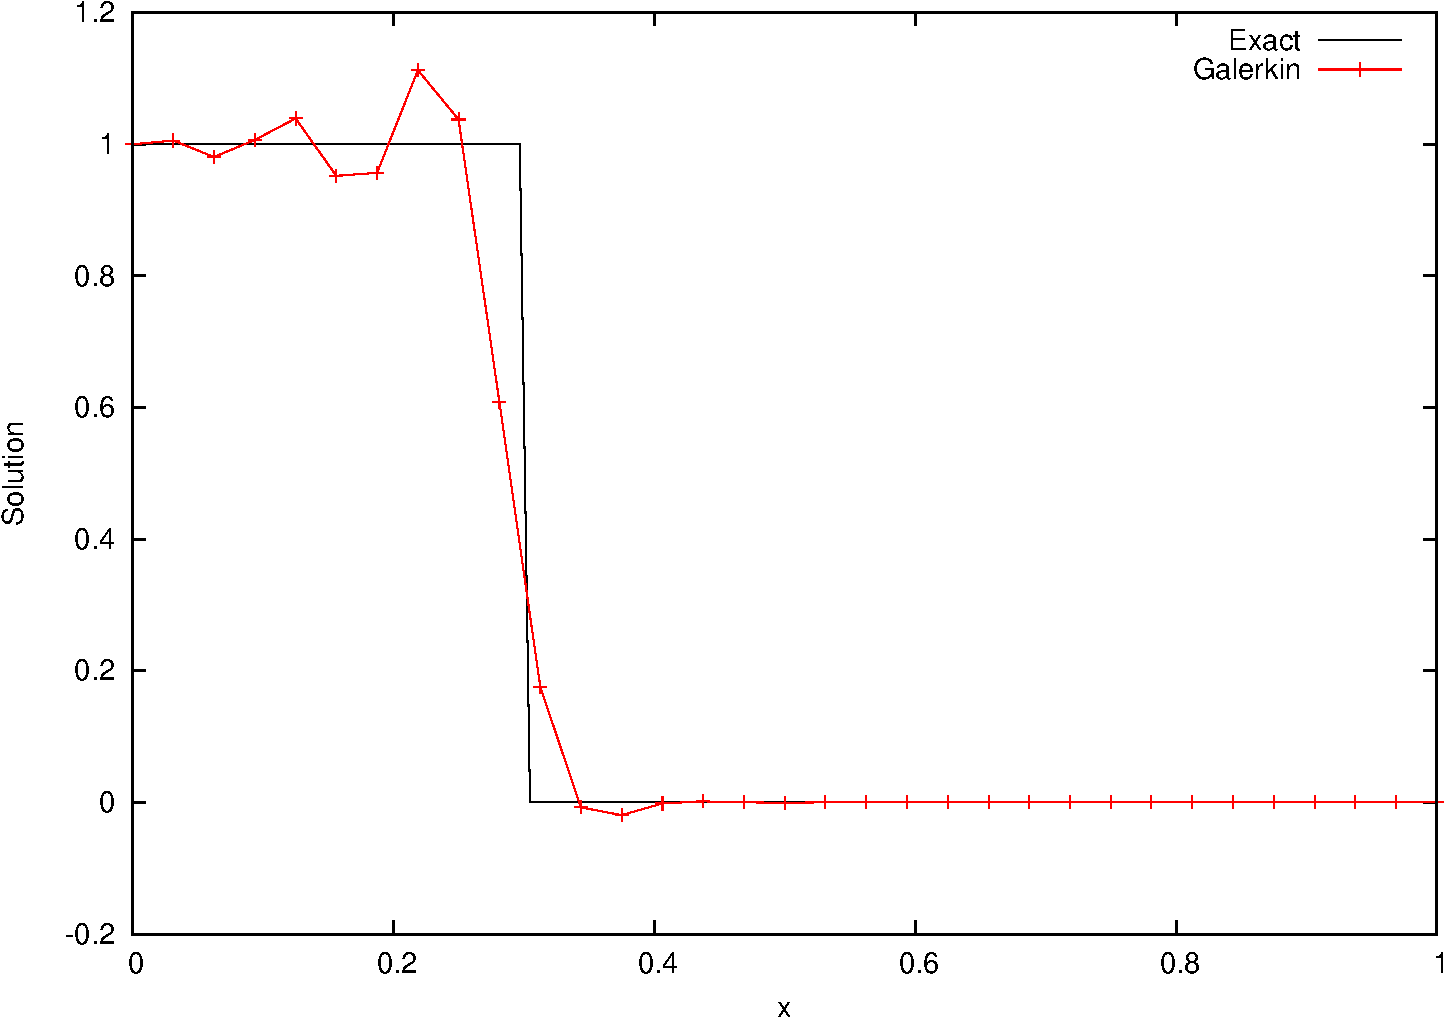
\includegraphics[height=0.6\textheight]{./figures/advection_Galerkin.pdf}
\end{center}

\end{frame}
%%%%%%%%%%%%%%%%%%%%%%%%%%%%%%%%%%%%%%%%%%%%%%%%%%%%%%%%%%%%%%%%%%%%%%%%%%%%%%%%%
\begin{frame}
\frametitle{Motivation}

\begin{itemize}
  \item The issue of spurious oscillations in conservation law problems has
    been extensively addressed in other spatial discretizations (finite difference,
    finite volume) via slope limiters, flux limiters, etc.
  \item Recently, efforts addressing this issue for the continuous finite
    element method (CFEM) have begun.
  \begin{itemize}
    \item CFEM is attractive due to the ability to model complex domains.
  \end{itemize}
  \item These oscillations give rise to unstable algorithms, where they grow
    without bound.
  \item Negativities can wreak havoc in a numerical algorithm and often
    cause simulations to terminate prematurely.
\end{itemize}

\end{frame}
%%%%%%%%%%%%%%%%%%%%%%%%%%%%%%%%%%%%%%%%%%%%%%%%%%%%%%%%%%%%%%%%%%%%%%%%%%%%%%%%%
\subsection{Objectives}
%%%%%%%%%%%%%%%%%%%%%%%%%%%%%%%%%%%%%%%%%%%%%%%%%%%%%%%%%%%%%%%%%%%%%%%%%%%%%%%%%
\begin{frame}
\frametitle{Objectives}

\begin{itemize}
   \item The objectives of this research are the following:
   \begin{itemize}
      \item \textcolor{secondarycolorheavy}{Accurately solve conservation law
        problems} using the continuous finite element method (CFEM).
      \begin{itemize}
        \item 2nd-order-accuracy in space (for smooth problems) is sought.
      \end{itemize}
      \item \textcolor{secondarycolorheavy}{Prevent spurious oscillations}.
      \begin{itemize}
	\item Complete immunity to spurious oscillations remains a dream for
          high-order schemes, but quality results are possible in practice.
      \end{itemize}
      \item \textcolor{secondarycolorheavy}{Prevent negativities}
        for physically non-negative quantities.
   \end{itemize}
\end{itemize}

\end{frame}
%%%%%%%%%%%%%%%%%%%%%%%%%%%%%%%%%%%%%%%%%%%%%%%%%%%%%%%%%%%%%%%%%%%%%%%%%%%%%%%%%
\subsection{FCT Introduction}
%%%%%%%%%%%%%%%%%%%%%%%%%%%%%%%%%%%%%%%%%%%%%%%%%%%%%%%%%%%%%%%%%%%%%%%%%%%%%%%%%
\begin{frame}
\frametitle{Introduction to Flux-Corrected Transport (FCT)}

\begin{itemize}
   \item Initially developed in 1973 for finite difference discretizations of
      transport/conservation law problems and recently applied to finite element
      method.
   \item Works by adding conservative fluxes to satisfy physical bounds on the
      solution.
   \item Employs a high-order scheme and a low-order, monotone scheme.
   \item Defines a \emph{correction}, or \emph{antidiffusion}, flux, which
      when added to the low-order scheme, produces the high-order scheme
      solution.
   \item Limits this correction flux to enforce the physical bounds imposed.
\end{itemize}

\end{frame}
%%%%%%%%%%%%%%%%%%%%%%%%%%%%%%%%%%%%%%%%%%%%%%%%%%%%%%%%%%%%%%%%%%%%%%%%%%%%%%%%%
\subsection{Outline}
%%%%%%%%%%%%%%%%%%%%%%%%%%%%%%%%%%%%%%%%%%%%%%%%%%%%%%%%%%%%%%%%%%%%%%%%%%%%%%%%%
\begin{frame}
\frametitle{Outline}

\begin{itemize}
   \item The scalar case
   \begin{itemize}
      \item Problem formulation
      \item Low-order, DMP-satisfying, positivity-preserving scheme
      \item High-order, entropy-based scheme
      \item High-order, DMP-satisfying, positivity-preserving FCT scheme
      \item Scalar results
   \end{itemize}
   \item The systems case (using the shallow water equations)
   \begin{itemize}
      \item Problem formulation
      \item Low-order, domain-invariant, positivity-preserving scheme
      \item High-order, entropy-based scheme
      \item High-order, LED, positivity-preserving FCT scheme
      \item Preliminary systems results
   \end{itemize}
   \item Conclusions
\end{itemize}

\end{frame}
%%%%%%%%%%%%%%%%%%%%%%%%%%%%%%%%%%%%%%%%%%%%%%%%%%%%%%%%%%%%%%%%%%%%%%%%%%%%%%%%%
\section{Scalar Introduction}
\subsection{Model}
%%%%%%%%%%%%%%%%%%%%%%%%%%%%%%%%%%%%%%%%%%%%%%%%%%%%%%%%%%%%%%%%%%%%%%%%%%%%%%%%%
\begin{frame}
\frametitle{Scalar Conservation Law Model}

\begin{itemize}
  \item This research first considers the following conservation law model:
    \begin{equation}
      \pd{\scalarsolution}{t} + \nabla\cdot\consflux(\scalarsolution)
      + \reactioncoef(\x)\scalarsolution\xt = \scalarsource\xt \eqc
    \end{equation}
    where $\reactioncoef(\x)\ge 0$ and $\scalarsource\xt\ge 0$.
  \item Some examples of applicability include
    \begin{itemize}
      \item \textcolor{secondarycolorheavy}{Linear advection}:
        advection of some quantity, such as a tracer
      \item \textcolor{secondarycolorheavy}{Traffic flow}:
        vehicle density on a one-lane highway
      \item \textcolor{secondarycolorheavy}{Inviscid Burgers' equation}:
        inviscid fluid flow model capturing some key features of gas dynamics
    \end{itemize}
  \item This model can be applied to radiation transport using source iteration:
    $\scalarsource\xt$ would include scattering source from the previous solution iterate.
\end{itemize}

\end{frame}
%%%%%%%%%%%%%%%%%%%%%%%%%%%%%%%%%%%%%%%%%%%%%%%%%%%%%%%%%%%%%%%%%%%%%%%%%%%%%%%%%
\section{Scalar Methodology}
\subsection{Problem Formulation}
%%%%%%%%%%%%%%%%%%%%%%%%%%%%%%%%%%%%%%%%%%%%%%%%%%%%%%%%%%%%%%%%%%%%%%%%%%%%%%%%%
\begin{frame}
\frametitle{Scalar Problem Formulation}

\begin{itemize}
  \item Consider a linear conservation law model
    ($\consflux(\scalarsolution)=\velocity\scalarsolution$):
    \begin{equation}
      \pd{\scalarsolution}{t} + \nabla\cdot(\velocity\scalarsolution)
      + \reactioncoef(\x)\scalarsolution\xt = \scalarsource\xt \eqc
    \end{equation}
    where $\reactioncoef(\x)\ge 0$ and $\scalarsource\xt\ge 0$.
  \item Complete problem by providing initial conditions and some boundary
    condition, such as Dirichlet:
   \begin{equation}
      u(\x,0) = u^0(\x) \quad \forall \x\in \domain
   \end{equation}
   \begin{equation}
      u\xt = u^{\text{inc}}(\x) \quad \forall \x\in \incomingdomainboundary
   \end{equation}
   \item CFEM solution:
   \begin{equation}
      \approximatescalarsolution\xt = \sum\limits_{j=1}^N U_j(t) \testfunction_j(\x) \eqc
      \quad \testfunction_j(\x)\in P^1_h
   \end{equation}
\end{itemize}

\end{frame}
%%%%%%%%%%%%%%%%%%%%%%%%%%%%%%%%%%%%%%%%%%%%%%%%%%%%%%%%%%%%%%%%%%%%%%%%%%%%%%%%
\subsection{Discretization}
%%%%%%%%%%%%%%%%%%%%%%%%%%%%%%%%%%%%%%%%%%%%%%%%%%%%%%%%%%%%%%%%%%%%%%%%%%%%%%%%
\begin{frame}
\frametitle{Discretization}

\begin{itemize}
   \item The simplest time discretization is forward Euler (FE), which gives the
      discrete system
   \begin{equation}
      \consistentmassmatrix\frac{\solutionvector^{n+1}-\solutionvector^n}
        {\dt} + \ssmatrix\solutionvector^n = \ssrhs^n \eqc
   \end{equation}
   where
   \begin{equation}
     M\ij^C \equiv \int\limits_{\support\ij}
       \testfunction_i(\x) \testfunction_j(\x) d\x \eqc
   \end{equation}
   \begin{equation}
     A\ij \equiv \int\limits_{\support\ij}\left(
       \mathbf{v}\cdot\nabla\testfunction_j(\x) +
		\reactioncoef(\x)\testfunction_j(\x)\right)\testfunction_i(\x) d\x \eqc
   \end{equation}
   \begin{equation}
      b_i^n \equiv \int\limits_{S_i} q(\x,t^n)\testfunction_i(\x) d\x \eqp
   \end{equation}
\end{itemize}

\end{frame}
%%%%%%%%%%%%%%%%%%%%%%%%%%%%%%%%%%%%%%%%%%%%%%%%%%%%%%%%%%%%%%%%%%%%%%%%%%%%%%%%%
\subsection{Low-Order Scheme}
%%%%%%%%%%%%%%%%%%%%%%%%%%%%%%%%%%%%%%%%%%%%%%%%%%%%%%%%%%%%%%%%%%%%%%%%%%%%%%%%%
\begin{frame}
\frametitle{Low-Order Scheme}

\begin{itemize}
   \item To get the low-order scheme, one does the following:
   \begin{itemize}
      \item Lumps the mass matrix:
        $\consistentmassmatrix\rightarrow\lumpedmassmatrix$.
      \item Adds a low-order diffusion operator:
        $\ssmatrix \rightarrow \ssmatrix+\loworderdiffusionmatrix$.
   \end{itemize}
   \item This gives the following, where $\solutionvector^{L,n+1}$ is the
     low-order solution:
   \begin{equation}
      \lumpedmassmatrix\frac{\solutionvector^{L,n+1}-\solutionvector^n}{\dt}
        + (\ssmatrix + \diffusionmatrix^L)\solutionvector^n = \ssrhs^n \eqp
   \end{equation}
   \item The diffusion matrix $\diffusionmatrix^L$ is assembled elementwise,
      where $K$ denotes an element, using a local bilinear form $b_K$ and a
      local low-order viscosity $\nu_K^L$:
   \begin{equation}
      D\ij^L = \sumKSij \nu_K^L b_K(\testfunction_j,\testfunction_i) \eqp
   \end{equation}
\end{itemize}

\end{frame}
%%%%%%%%%%%%%%%%%%%%%%%%%%%%%%%%%%%%%%%%%%%%%%%%%%%%%%%%%%%%%%%%%%%%%%%%%%%%%%%%%
\begin{frame}
\frametitle{Local Viscous Bilinear Form}

\begin{itemize}
   \item The local bilinear form is defined as follows, where $|K|$ denotes
      the volume of element $K$, $\mathcal{I}(K)$ is the set of indices
      corresponding to degrees of freedom with nonempty support on $K$, and
      $n_K$ is the cardinality of this set.
   \begin{equation}
      b_K(\testfunction_j, \testfunction_i) \equiv \left\{\begin{array}{l l}
         -\frac{1}{n_K - 1}\cellvolume & i\ne j, \quad i,j\in \mathcal{I}(K)\\
         \cellvolume                   & i = j,  \quad i,j\in \mathcal{I}(K)\\
         0                & i\notin\mathcal{I}(K)\,|\, j\notin\mathcal{I}(K)
      \end{array}\right. \eqp
   \end{equation}
   \item Some properties that result from this definition are
   \begin{equation}
      \sum\limits_j b_K(\testfunction_j, \testfunction_i) = 0 \eqc
   \end{equation}
   \begin{equation}
      b_K(\testfunction_i, \testfunction_i) > 0 \eqp
   \end{equation}
\end{itemize}

\end{frame}
%%%%%%%%%%%%%%%%%%%%%%%%%%%%%%%%%%%%%%%%%%%%%%%%%%%%%%%%%%%%%%%%%%%%%%%%%%%%%%%%%
\begin{frame}
\frametitle{Low-Order Viscosity}

\begin{itemize}
   \item The low-order viscosity is defined as
   \begin{equation}
     \lowordercellviscosity[\timeindex] \equiv \max\limits_{i\ne j\in\indicescell}
     \frac{\max(0,\ssmatrixletter\ij^\timeindex)}
     {-\mkern-20mu\sumKSij[T]\mkern-20mu\localviscbilinearform{T}{j}{i}}
     \eqp
   \end{equation}
   \item This definition is designed to be the smallest number such that the
      following is guaranteed:
   \begin{equation}
      D^L\ij \leq -A\ij, \quad j\ne i \eqp
   \end{equation}
   \item This is used to guarantee that the low-order steady-state matrix
      $\ssmatrix^L=\ssmatrix+\diffusionmatrix^L$ is an M-matrix, i.e., a \emph{monotone} matrix:
      $\ssmatrix^L\solutionvector \ge 0\Rightarrow \solutionvector\ge 0$.
\end{itemize}

\end{frame}
%%%%%%%%%%%%%%%%%%%%%%%%%%%%%%%%%%%%%%%%%%%%%%%%%%%%%%%%%%%%%%%%%%%%%%%%%%%%%%%%%
\begin{frame}
\frametitle{Discrete Maximum Principle}

\begin{itemize}
   \item In addition to guaranteeing monotonicity and positivity, the low-order
      viscous terms guarantee the following discrete maximum principle (DMP),
      where $U^n_{\max,i} = \max\limits_{j\in\mathcal{I}(S_i)}U^n_j$,
      $U^n_{\min,i} = \min\limits_{j\in\mathcal{I}(S_i)}U^n_j$:
      \begin{equation}
         W_i^-\leq
         U_i^{L,n+1}\leq
         W_i^+\qquad\forall i \eqc
      \end{equation}
      \begin{equation}
         W_i^\pm \equiv U_{\substack{\max\\\min},i}^n\left(
         1-\frac{\dt}{M_{i,i}^L}
         \sum\limits_j A\ij^L\right)
         + \frac{\Delta t}{M_{i,i}^L}b_i^n \eqp
      \end{equation}
   \item For example, when there is no reaction term or source term, this reduces
      to the following DMP, which implies the scheme is local extremum
      diminishing (LED):
      \begin{equation}
         U^n_{\min,i}\leq
         U_i^{L,n+1}\leq
         U^n_{\max,i}\qquad\forall i \eqp
      \end{equation}
\end{itemize}

\end{frame}
%%%%%%%%%%%%%%%%%%%%%%%%%%%%%%%%%%%%%%%%%%%%%%%%%%%%%%%%%%%%%%%%%%%%%%%%%%%%%%%%%
\begin{frame}
\frametitle{Low-Order Scheme Results Example}

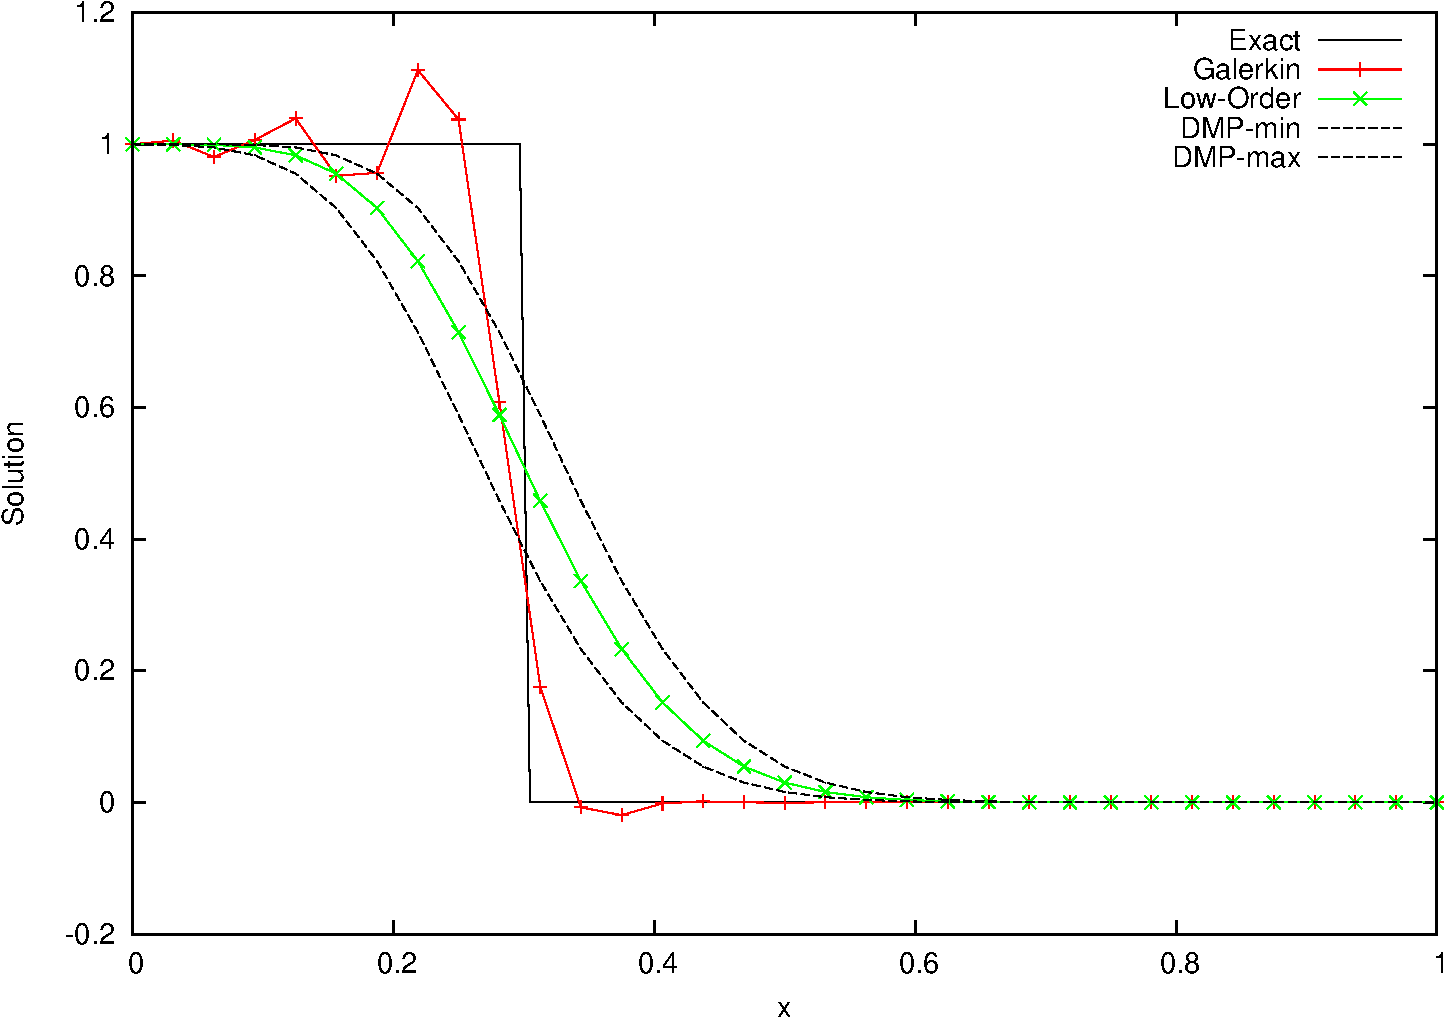
\includegraphics[width=\textwidth]{./figures/advection_low_order.pdf}

\end{frame}
%%%%%%%%%%%%%%%%%%%%%%%%%%%%%%%%%%%%%%%%%%%%%%%%%%%%%%%%%%%%%%%%%%%%%%%%%%%%%%%%%
\subsection{High-Order Scheme}
%%%%%%%%%%%%%%%%%%%%%%%%%%%%%%%%%%%%%%%%%%%%%%%%%%%%%%%%%%%%%%%%%%%%%%%%%%%%%%%%%
\begin{frame}
\frametitle{Introduction to Entropy Viscosity}

\begin{itemize}
   \item The standard Galerkin CFEM weak solution is not unique. Even with
      FCT, it would not necessarily converge to the correct, physical
      weak solution, i.e., the \emph{entropy} solution.
   \item To converge to the entropy solution, one must ensure that an entropy
      inequality is satisfied:
      \begin{equation}
         R(u) \equiv \pd{\eta(u)}{t} + \nabla\cdot\mathbf{f}^\eta(u) \leq 0
      \end{equation}
      for any convex entropy $\eta(u)$ and corresponding entropy flux
      $\mathbf{f}^\eta(u)$.
   \item This \emph{entropy residual} $R(u)$ measures entropy production;
      where it is positive, the inequality is violated, so the residual
      should be decreased somehow.
   \item To enforce the inequality, the entropy viscosity method adds
      viscosity in proportion to local entropy production, thus decreasing
      local entropy.
\end{itemize}

\end{frame}
%%%%%%%%%%%%%%%%%%%%%%%%%%%%%%%%%%%%%%%%%%%%%%%%%%%%%%%%%%%%%%%%%%%%%%%%%%%%%%%%%
\begin{frame}
\frametitle{Entropy Viscosity Definition}

\begin{itemize}
   \item One chooses a convex entropy function $\eta(u)$ such
   as $\eta(u)=\frac{1}{2}u^2$ and manipulates the
   conservation law equation to get an entropy residual:
   \begin{equation}
      R(u) = \pd{\eta}{t}
      + \frac{d\eta}{du}\left(\nabla\cdot(\mathbf{v}u)
      + \reactioncoef u 
      - q \right) \eqp
   \end{equation}
   \item Viscosity is set to be proportional to a linear combination
      of the local entropy residual $R_K(u) = \left\|R(u)\right\|_{L^\infty(K)}$
      and entropy jumps $J_F(u)$ across the faces:
      \begin{equation}
         \nu^{\eta}_K \propto c_R R_K(u_h)
         + c_J\max\limits_{F\in\partial K}J_F(u_h) \eqp
      \end{equation}
   \item In practice, the entropy viscosity becomes the following, where the
      denominator is just a normalization constant:
      \begin{equation}
         \nu^{\eta}_K = \frac{c_R R_K(u_h)
         + c_J\max\limits_{F\in\partial K}J_F(u_h)}
         {\|\eta(u_h)-\bar{\eta}(u_h)\|_{L^\infty(\mathcal{D})}} \eqp
      \end{equation}
\end{itemize}
   
\end{frame}
%%%%%%%%%%%%%%%%%%%%%%%%%%%%%%%%%%%%%%%%%%%%%%%%%%%%%%%%%%%%%%%%%%%%%%%%%%%%%%%%%
\begin{frame}
\frametitle{High-Order Scheme}

\begin{itemize}
   \item The high-order viscosity does not need to be any greater than the
      low-order viscosity:
      \begin{equation}
         \nu^{H,n}_K = \min(\nu^{L}_K,\nu^{\eta,n}_K) \eqp
      \end{equation}
   \item For the high-order scheme, the mass matrix is not modified; the
      only change is the addition of the high-order diffusion operator
      $\diffusionmatrix^{H,n}$:
      $\ssmatrix \rightarrow \ssmatrix + \diffusionmatrix^{H,n}$:
      \begin{equation}
        \consistentmassmatrix\frac{\solutionvector^{H,n+1}
          -\solutionvector^n}{\dt} + (\ssmatrix + \diffusionmatrix^{H,n})
          \solutionvector^n = \ssrhs^n \eqp
      \end{equation}
   \item The high-order diffusion matrix is computed just as the low-order
      counterpart, except that $\nu^{H,n}_K$ is used instead of $\nu^{L}_K$:
      \begin{equation}
         D\ij^{H,n} = \sum\limits_{K\subset S\ij}\nu_K^{H,n}
            b_K(\testfunction_j,\testfunction_i) \eqp
      \end{equation}
\end{itemize}

\end{frame}
%%%%%%%%%%%%%%%%%%%%%%%%%%%%%%%%%%%%%%%%%%%%%%%%%%%%%%%%%%%%%%%%%%%%%%%%%%%%%%%%%
\begin{frame}
\frametitle{High-Order Scheme Results Example}

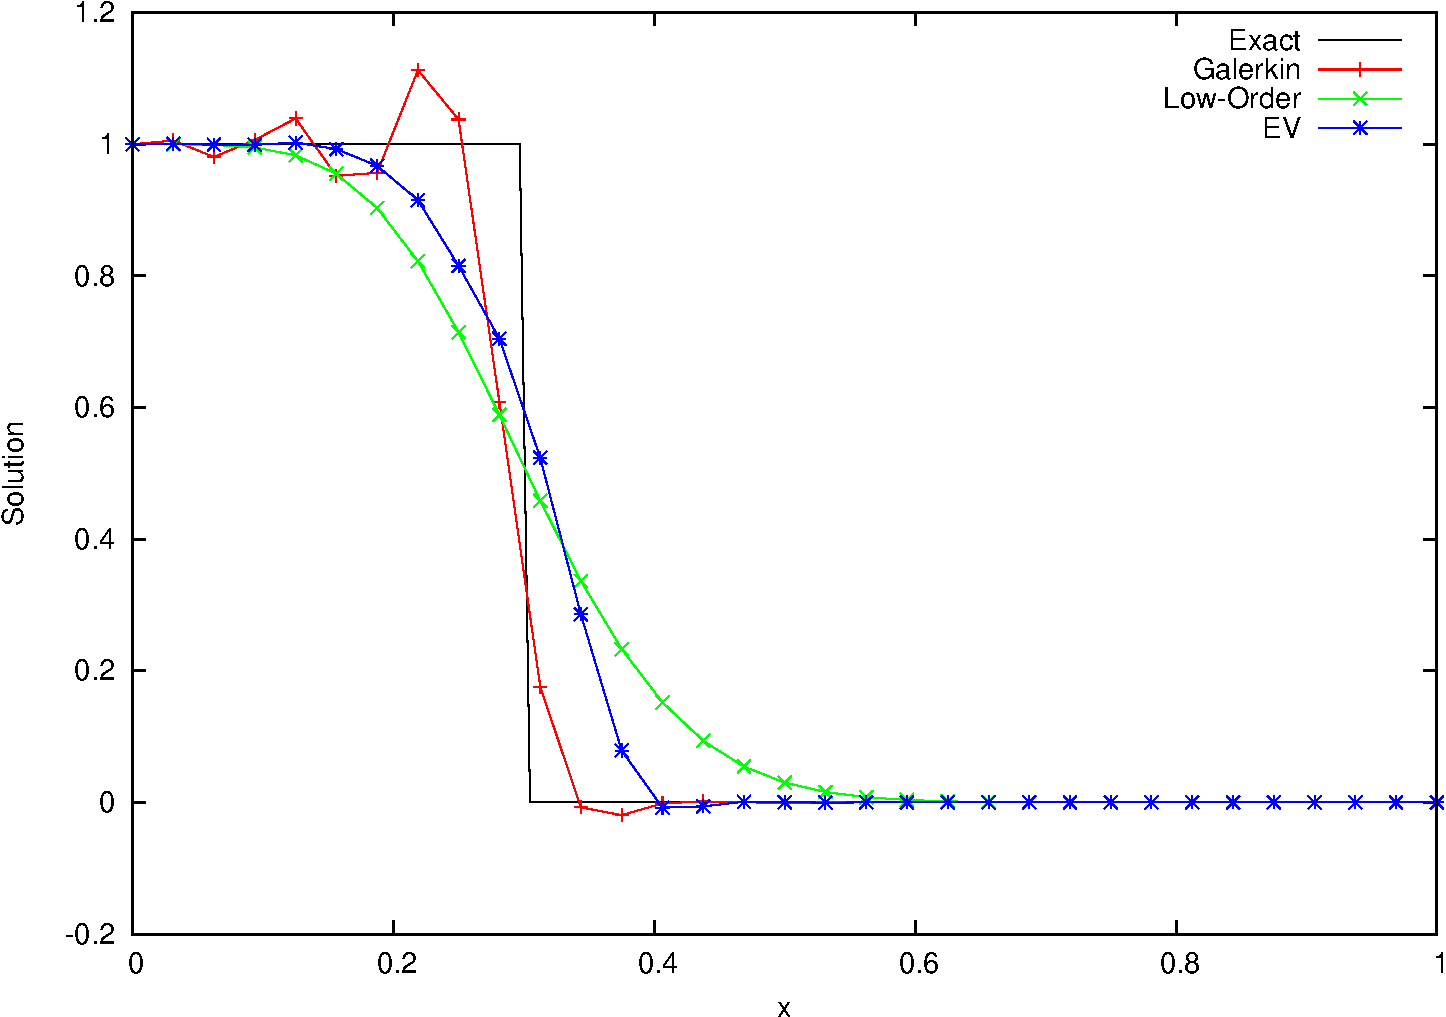
\includegraphics[width=\textwidth]{./figures/advection_high_order.pdf}

\end{frame}
%%%%%%%%%%%%%%%%%%%%%%%%%%%%%%%%%%%%%%%%%%%%%%%%%%%%%%%%%%%%%%%%%%%%%%%%%%%%%%%%%
\subsection{FCT Scheme}
%%%%%%%%%%%%%%%%%%%%%%%%%%%%%%%%%%%%%%%%%%%%%%%%%%%%%%%%%%%%%%%%%%%%%%%%%%%%%%%%%
\begin{frame}
\frametitle{FCT Antidiffusive Flux Definition}

\begin{itemize}
   \item Recall that FCT defines antidiffusive correction fluxes
      from a low-order, monotone scheme to a high-order scheme. Calling
      these fluxes $\correctionfluxvector$, this gives
      \begin{equation}
        \lumpedmassmatrix\frac{\solutionvector^{H,n+1}-\solutionvector^n}{\dt}
          + (\ssmatrix+\diffusionmatrix^L)\solutionvector^n = \ssrhs^n
          + \correctionfluxvector \eqp
      \end{equation}
   \item Subtracting the high-order scheme equation from this gives the
      definition of $\correctionfluxvector$:
      \begin{equation}
        \correctionfluxvector \equiv
          -(\consistentmassmatrix-\lumpedmassmatrix)
          \frac{\solutionvector^{H,n+1}-\solutionvector^n}{\dt}
          + (\diffusionmatrix^L-\diffusionmatrix^{H,n})\solutionvector^n \eqp
      \end{equation}
   \item Decomposing $\correctionfluxvector$ into internodal fluxes
      $\correctionfluxij$ such that $\sum_j \correctionfluxij =
      \correctionfluxletter_i$, where $\Delta_{j,i}[\mathbf{y}]$
      denotes $y_j - y_i$:
   \begin{equation}
     \correctionfluxij = -M\ij^C\Delta_{j,i}\left[
       \frac{\solutionvector^{H,n+1}-\solutionvector^n}{\Delta t}\right]
       + (D\ij^L-D\ij^{H,n})\Delta_{j,i}[\solutionvector^n] \eqp
   \end{equation}
\end{itemize}

\end{frame}
%%%%%%%%%%%%%%%%%%%%%%%%%%%%%%%%%%%%%%%%%%%%%%%%%%%%%%%%%%%%%%%%%%%%%%%%%%%%%%%%%
\begin{frame}
\frametitle{FCT Scheme Overview}

\begin{itemize}
   \item Recall that the objective of FCT is to limit these antidiffusive
      fluxes to enforce some physical bounds.
   \item The chosen bounds take the form of the DMP satisfied by the
      low-order scheme:
      \begin{equation}
         W_i^-\leq
         U_i^{n+1}\leq
         W_i^+\qquad\forall i \eqp
      \end{equation}
   \item This is achieved by applying a limiting coefficient $L\ij$ to each
      internodal flux $\correctionfluxij$:
      \begin{equation}
        \lumpedmassmatrix\frac{\solutionvector^{n+1}-\solutionvector^n}{\dt}
          + \ssmatrix^L\solutionvector^n = \ssrhs
          + \limitermatrix\cdot\correctionfluxmatrix \eqp
      \end{equation}
   \item Each limiting coefficient is between zero and unity: $0\leq L\ij\leq 1$.
   \begin{itemize}
      \item If all $L\ij$ are zero, then the low-order scheme is produced.
      \item If all $L\ij$ are one, then the high-order scheme is produced.
   \end{itemize}
\end{itemize}

\end{frame}
%%%%%%%%%%%%%%%%%%%%%%%%%%%%%%%%%%%%%%%%%%%%%%%%%%%%%%%%%%%%%%%%%%%%%%%%%%%%%%%%%
\begin{frame}
\frametitle{Limiting Coefficients Introduction}

\begin{itemize}
   \item The enforced bounds can be rearranged to bound the limited flux sums:
      \begin{equation}
         Q^-_i \leq \sum\limits_j L\ij \correctionfluxij \leq Q^+_i \eqc
      \end{equation}
      where $Q_i^\pm$ has the following definition:
      \begin{equation}
         Q_i^\pm \equiv M_{i,i}^L\frac{W_i^\pm-U_i^n}{\Delta t}
         + \sum\limits_j A_{i,j}^L U_j^n - b_i \eqp
      \end{equation}
   \item The classic Zalesak limiting strategy starts by separating the
      negative and positive fluxes:
      \begin{equation}
         Q^-_i \leq \sum\limits_{j:\correctionfluxij<0} L\ij \correctionfluxij +
            \sum\limits_{j:\correctionfluxij>0} L\ij \correctionfluxij\leq Q^+_i \eqp
      \end{equation}
      The positive fluxes risk violating $Q_i^+$, and the negative fluxes risk
      violating $Q_i^-$.
\end{itemize}

\end{frame}
%%%%%%%%%%%%%%%%%%%%%%%%%%%%%%%%%%%%%%%%%%%%%%%%%%%%%%%%%%%%%%%%%%%%%%%%%%%%%%%%%
\begin{frame}
\frametitle{Limiting Coefficients Definition}

\begin{itemize}
   \item Zalesak's limiting coefficients assume that
      all positive fluxes into a node $i$ have the same limiting coefficient
      $L^+_i$ and similarly, negative fluxes have the same limiting coefficient
      $L^-_i$:
      \begin{equation}
        Q^-_i \leq L^-_i \correctionfluxletter^-_i
          + L^+_i \correctionfluxletter^+_i \leq Q^+_i \eqp
      \end{equation}
      where
      \begin{equation}
        \correctionfluxletter_i^- \equiv \sum\limits_{j:\correctionfluxij<0}
          \correctionfluxij \eqc \qquad
        \correctionfluxletter_i^+ \equiv \sum\limits_{j:\correctionfluxij>0}
          \correctionfluxij \eqp
      \end{equation}
   \item As a conservative bound for $L^+_i$, contributions from negative fluxes
      are ignored (pretending $L_i^-=0$), giving
      $L^+_i \leq \frac{Q_i^+}{\correctionfluxletter_i^+}$
      and similarly for $L^-_i$ and the lower bound.
\end{itemize}

\end{frame}
%%%%%%%%%%%%%%%%%%%%%%%%%%%%%%%%%%%%%%%%%%%%%%%%%%%%%%%%%%%%%%%%%%%%%%%%%%%%%%%%%
\begin{frame}
\frametitle{Limiting Coefficients Definition (Cont.)}

\begin{itemize}
   \item Then, recalling that limiting coefficients are not greater than unity:
      \begin{equation}
         L_i^\pm \equiv\left\{
            \begin{array}{l l}
               1 & \correctionfluxletter_i^\pm = 0\\
               \min\left(1,\frac{Q_i^\pm}{\correctionfluxletter_i^\pm}\right) &
                 \correctionfluxletter_i^\pm \ne 0
            \end{array}
            \right. \eqp
      \end{equation}
   \item However, to limit fluxes conservatively, limited correction fluxes must
      be equal and opposite:
      \begin{equation}
        L\ij \correctionfluxij = -L_{j,i}
          \MakeUppercase{\correctionfluxletter}_{j,i} \eqp
      \end{equation}
      Since $\correctionfluxij$ happens to be skew symmetric
      ($\MakeUppercase{\correctionfluxletter}_{j,i}=-\correctionfluxij$) due to the
      chosen flux decomposition, the limiting coefficients must be symmetric:
      $L_{j,i} = L\ij$.
\end{itemize}

\end{frame}
%%%%%%%%%%%%%%%%%%%%%%%%%%%%%%%%%%%%%%%%%%%%%%%%%%%%%%%%%%%%%%%%%%%%%%%%%%%%%%%%%
\begin{frame}
\frametitle{Limiting Coefficients Definition (Cont.)}

\begin{itemize}
   \item Thus when deciding the limiting coefficient $L\ij$ for a flux $\correctionfluxij$, 
      one must not only consider the bounds for $i$ but also the bounds for $j$.
      Specifically, a positive flux $\correctionfluxij$ risks violating $Q_i^+$ and $Q_j^-$.
      Putting everything together,
      \begin{equation}
         L\ij \equiv\left\{
            \begin{array}{l l}
               \min(L_i^+,L_j^-) & \correctionfluxij \geq 0\\
               \min(L_i^-,L_j^+) & \correctionfluxij < 0
            \end{array}
            \right. \eqp
      \end{equation}
\end{itemize}

\end{frame}
%%%%%%%%%%%%%%%%%%%%%%%%%%%%%%%%%%%%%%%%%%%%%%%%%%%%%%%%%%%%%%%%%%%%%%%%%%%%%%%%%
\begin{frame}
\frametitle{FCT Scheme Results Example}

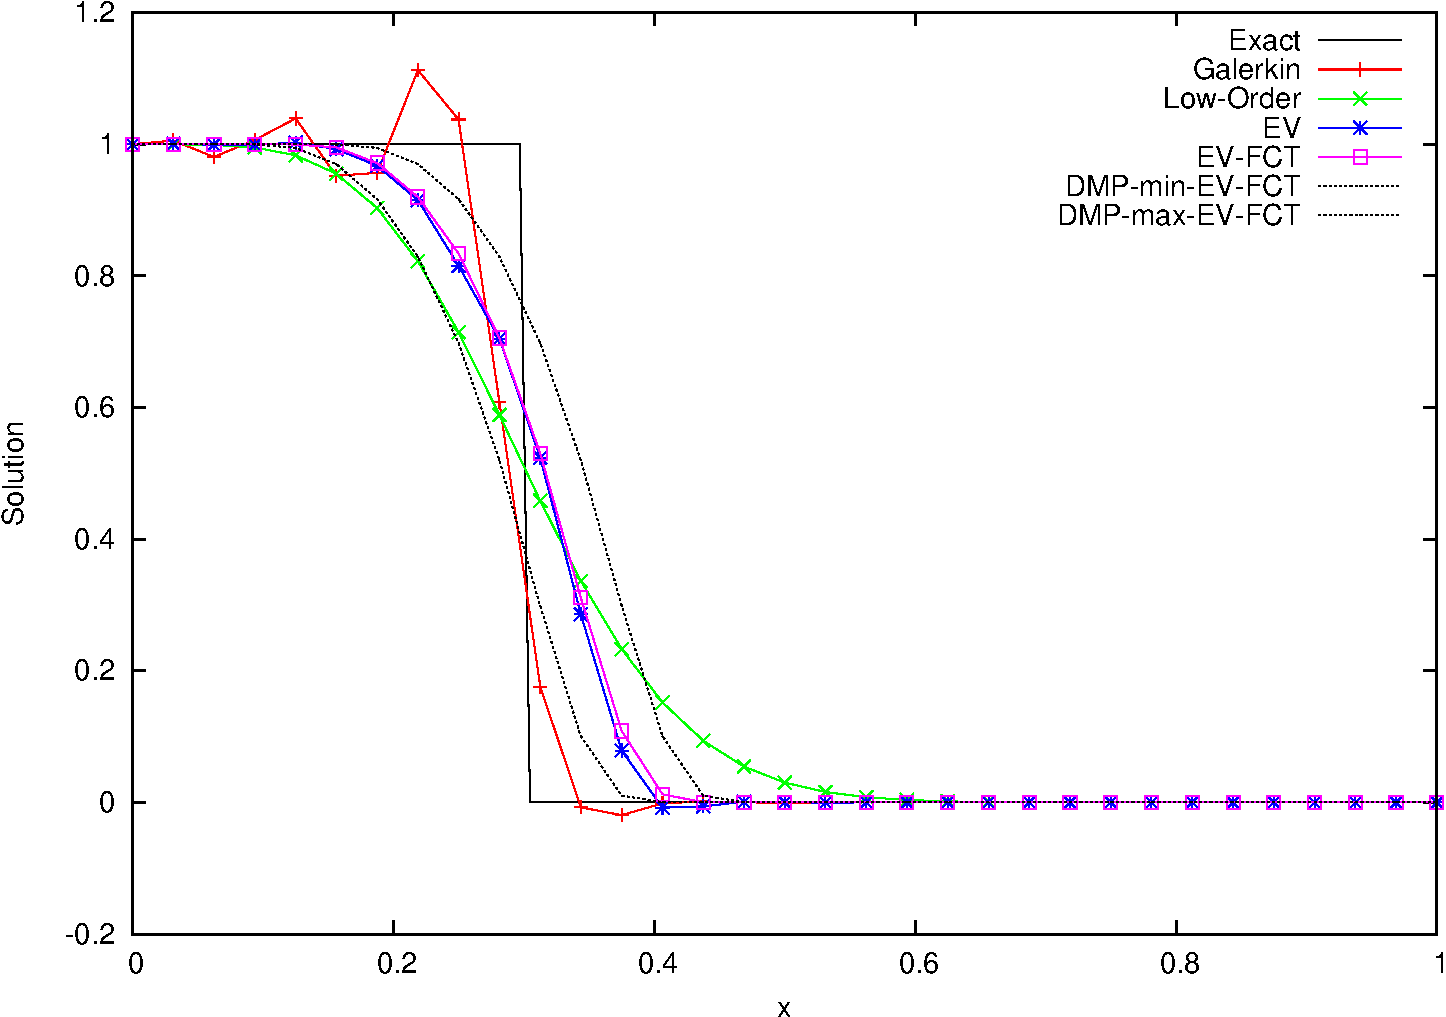
\includegraphics[width=\textwidth]{./figures/advection_FCT.pdf}

\end{frame}
%%%%%%%%%%%%%%%%%%%%%%%%%%%%%%%%%%%%%%%%%%%%%%%%%%%%%%%%%%%%%%%%%%%%%%%%%%%%%%%%%
\section{Scalar Results}
%%%%%%%%%%%%%%%%%%%%%%%%%%%%%%%%%%%%%%%%%%%%%%%%%%%%%%%%%%%%%%%%%%%%%%%%%%%%%%%%%
\begin{frame}
\frametitle{1-D Source Problem Results}

\begin{center}
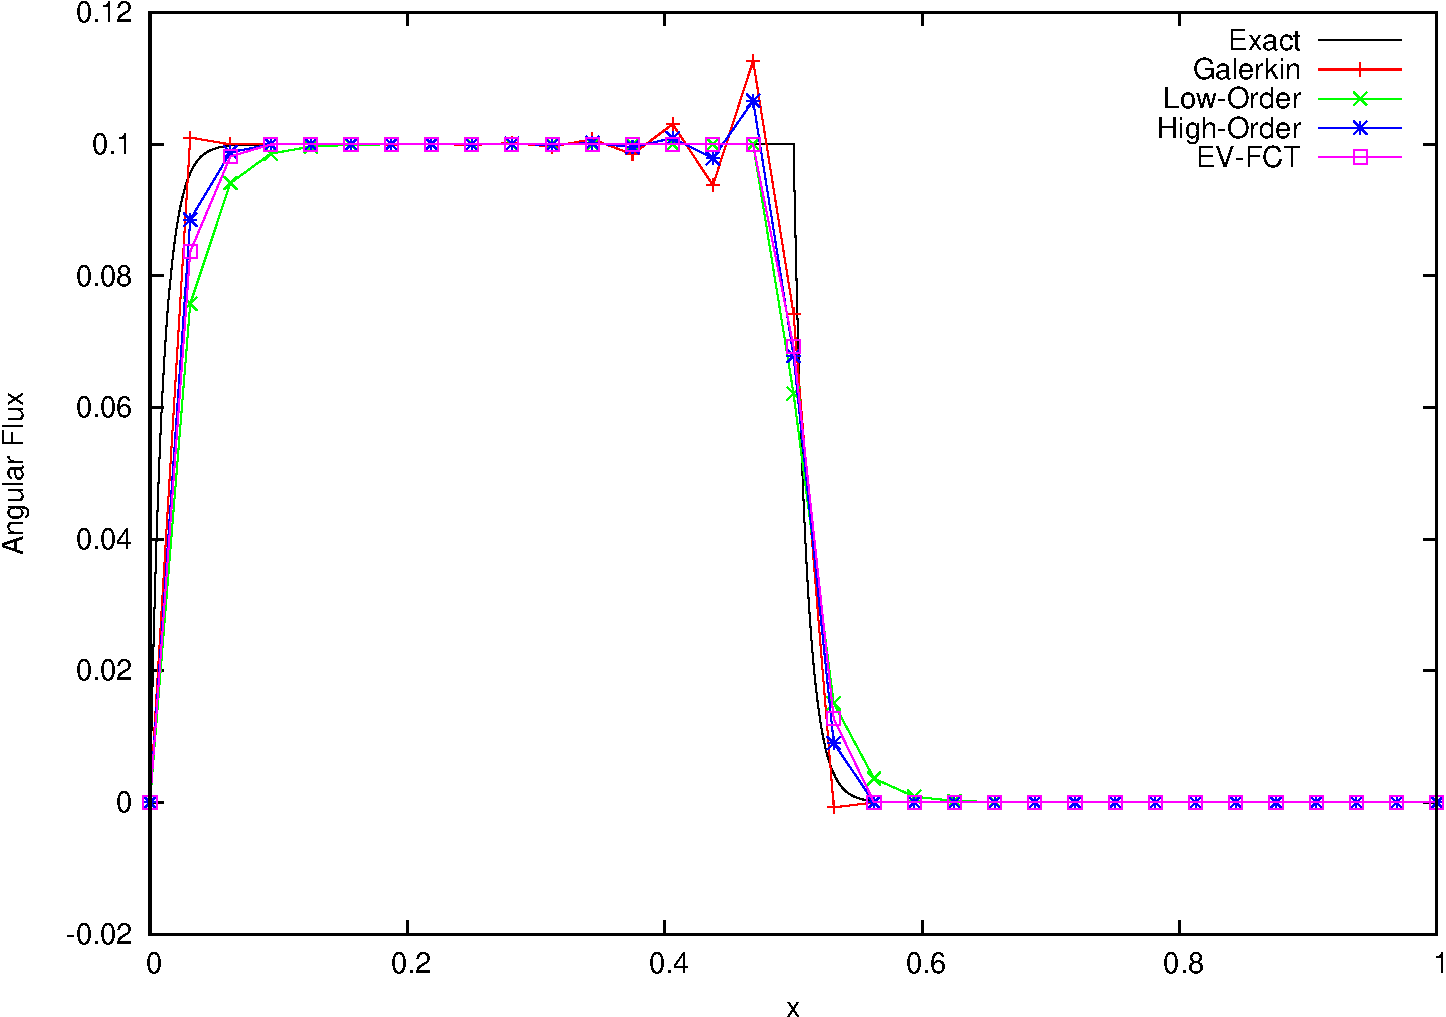
\includegraphics[height=0.8\textheight]{./figures/solutions_source_FE.pdf}
\end{center}

\end{frame}
%%%%%%%%%%%%%%%%%%%%%%%%%%%%%%%%%%%%%%%%%%%%%%%%%%%%%%%%%%%%%%%%%%%%%%%%%%%%%%%%%
\begin{frame}
\frametitle{2-D Void-to-Absorber Problem Results}

\begin{figure}[h]
   \centering
   \begin{subfigure}{0.3\textwidth}
      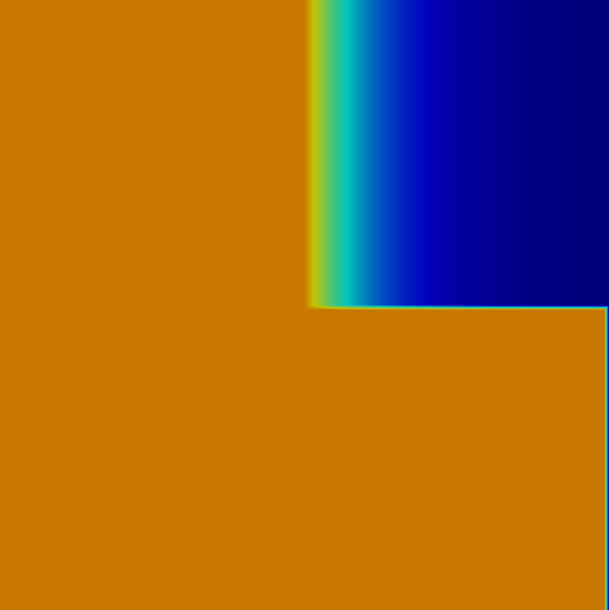
\includegraphics[width=0.8\textwidth]{./figures/exact.png}
      \caption{Exact}
   \end{subfigure}
   \begin{subfigure}{0.3\textwidth}
      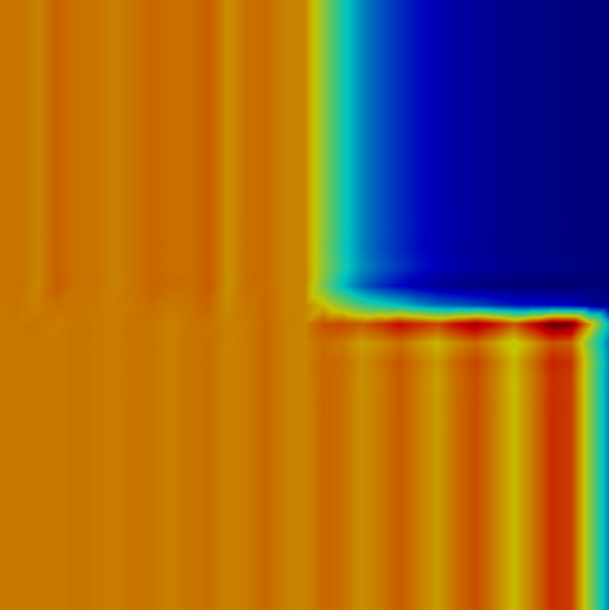
\includegraphics[width=0.8\textwidth]{./figures/Gal.png}
      \caption{Galerkin}
   \end{subfigure}
   \begin{subfigure}{0.3\textwidth}
      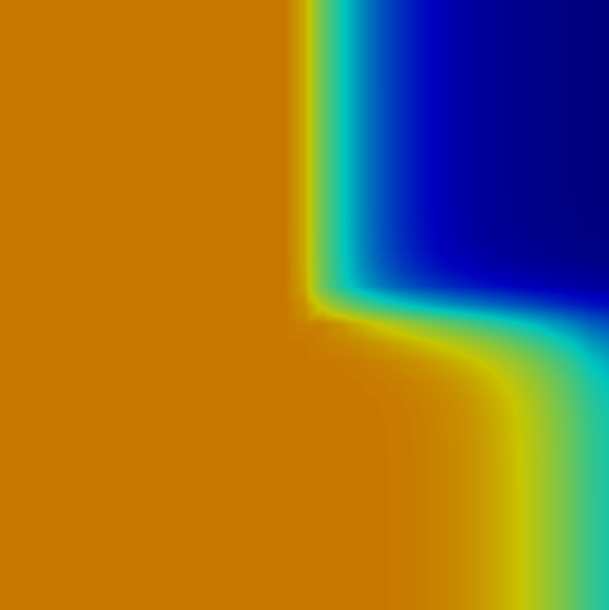
\includegraphics[width=0.8\textwidth]{./figures/GalFCT.png}
      \caption{Galerkin-FCT}
   \end{subfigure}
   \begin{subfigure}{0.3\textwidth}
      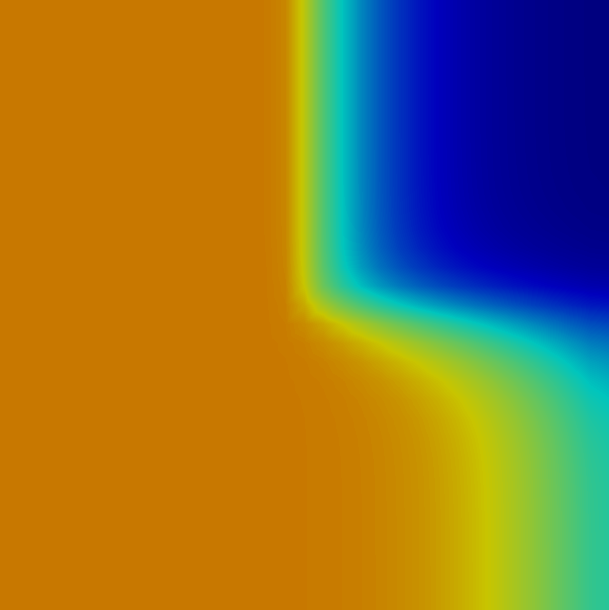
\includegraphics[width=0.8\textwidth]{./figures/low.png}
      \caption{Low-order}
   \end{subfigure}
   \begin{subfigure}{0.3\textwidth}
      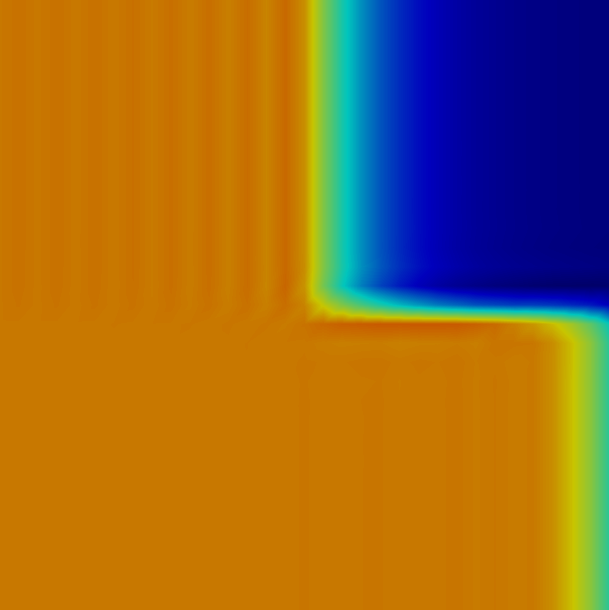
\includegraphics[width=0.8\textwidth]{./figures/EV.png}
      \caption{EV}
   \end{subfigure}
   \begin{subfigure}{0.3\textwidth}
      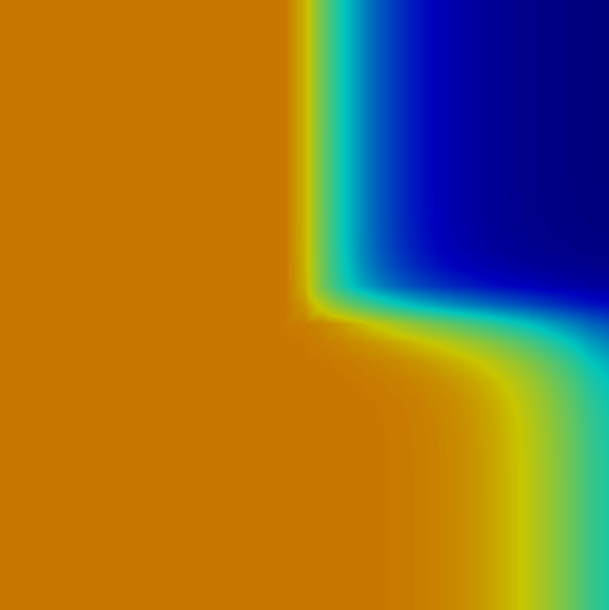
\includegraphics[width=0.8\textwidth]{./figures/EVFCT.png}
      \caption{EV-FCT}
   \end{subfigure}
\end{figure}

\end{frame}
%%%%%%%%%%%%%%%%%%%%%%%%%%%%%%%%%%%%%%%%%%%%%%%%%%%%%%%%%%%%%%%%%%%%%%%%%%%%%%%%%
\begin{frame}
\frametitle{3-D Void-to-Absorber Problem Results}

\begin{figure}[h]
   \centering
   \begin{subfigure}{0.45\textwidth}
      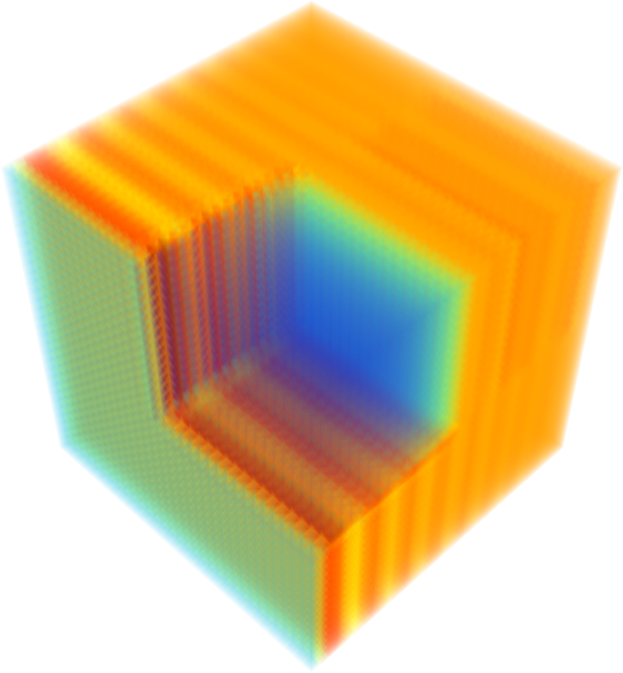
\includegraphics[width=\textwidth]{./figures/Gal_3D.png}
      \caption{Galerkin}
   \end{subfigure}
   \begin{subfigure}{0.45\textwidth}
      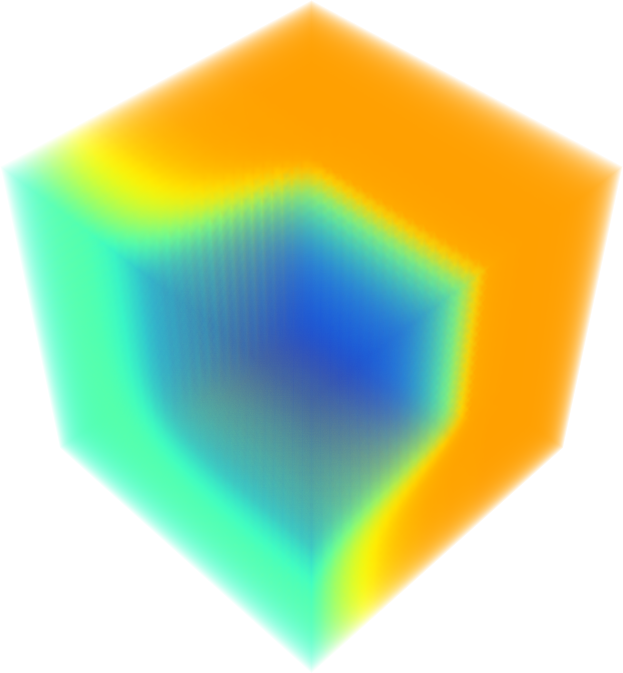
\includegraphics[width=\textwidth]{./figures/GalFCT_3D.png}
      \caption{Galerkin-FCT}
   \end{subfigure}
\end{figure}

\end{frame}
%%%%%%%%%%%%%%%%%%%%%%%%%%%%%%%%%%%%%%%%%%%%%%%%%%%%%%%%%%%%%%%%%%%%%%%%%%%%%%%%%
\begin{frame}
\frametitle{2-D Skew Void-to-Absorber Problem Results}

\begin{figure}[h]
   \centering
   \begin{subfigure}{0.3\textwidth}
      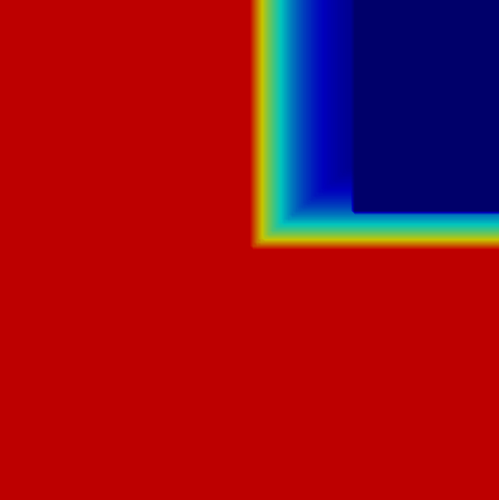
\includegraphics[width=0.8\textwidth]{./figures/skew_exact.png}
      \caption{Exact}
   \end{subfigure}
   \begin{subfigure}{0.3\textwidth}
      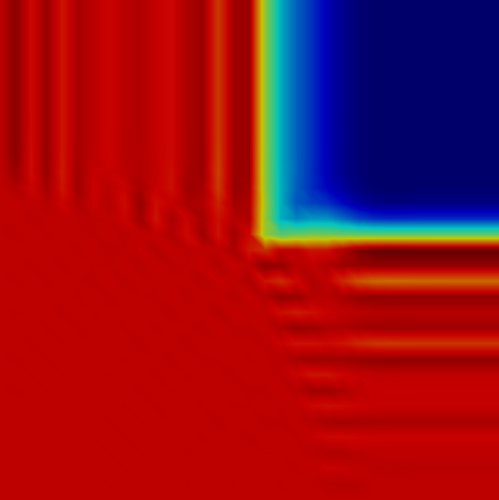
\includegraphics[width=0.8\textwidth]{./figures/skew_Gal.png}
      \caption{Galerkin}
   \end{subfigure}
   \begin{subfigure}{0.3\textwidth}
      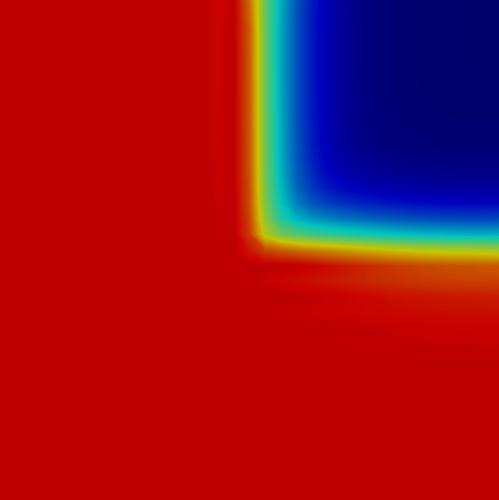
\includegraphics[width=0.8\textwidth]{./figures/skew_GalFCT.png}
      \caption{Galerkin-FCT}
   \end{subfigure}
   \begin{subfigure}{0.3\textwidth}
      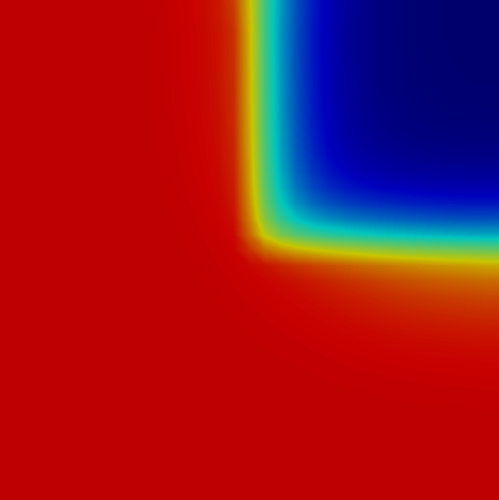
\includegraphics[width=0.8\textwidth]{./figures/skew_low.png}
      \caption{Low-order}
   \end{subfigure}
   \begin{subfigure}{0.3\textwidth}
      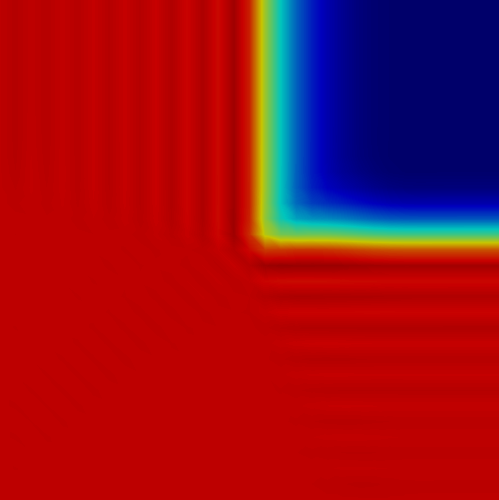
\includegraphics[width=0.8\textwidth]{./figures/skew_EV.png}
      \caption{EV}
   \end{subfigure}
   \begin{subfigure}{0.3\textwidth}
      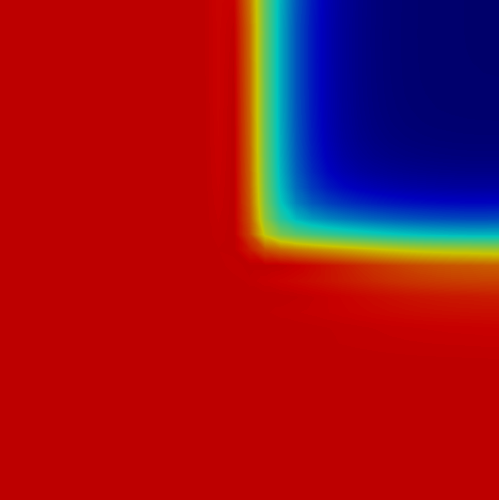
\includegraphics[width=0.8\textwidth]{./figures/skew_EVFCT.png}
      \caption{EV-FCT}
   \end{subfigure}
\end{figure}

\end{frame}
%%%%%%%%%%%%%%%%%%%%%%%%%%%%%%%%%%%%%%%%%%%%%%%%%%%%%%%%%%%%%%%%%%%%%%%%%%%%%%%%%
\begin{frame}
\frametitle{Galerkin-FCT Vs. EV-FCT}

\begin{center}
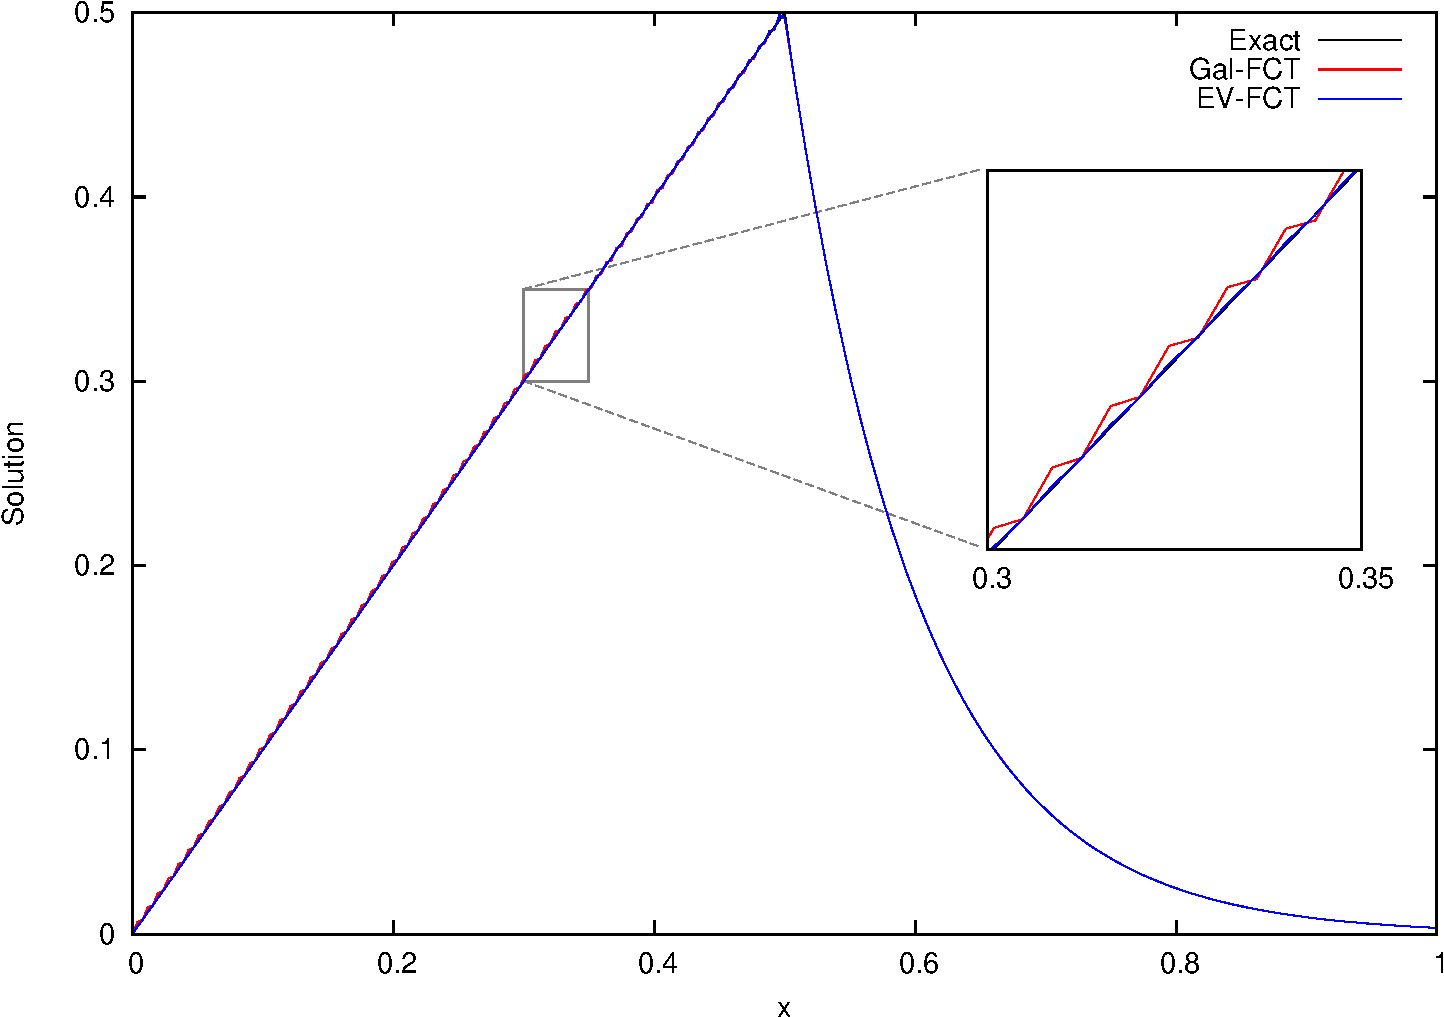
\includegraphics[height=0.8\textheight]{./figures/sourcevoid_FCT_comparison.pdf}
\end{center}

\end{frame}
%%%%%%%%%%%%%%%%%%%%%%%%%%%%%%%%%%%%%%%%%%%%%%%%%%%%%%%%%%%%%%%%%%%%%%%%%%%%%%%%%
\begin{frame}
\frametitle{1-D Smooth Problem Convergence Results (Using FE)}

\begin{center}
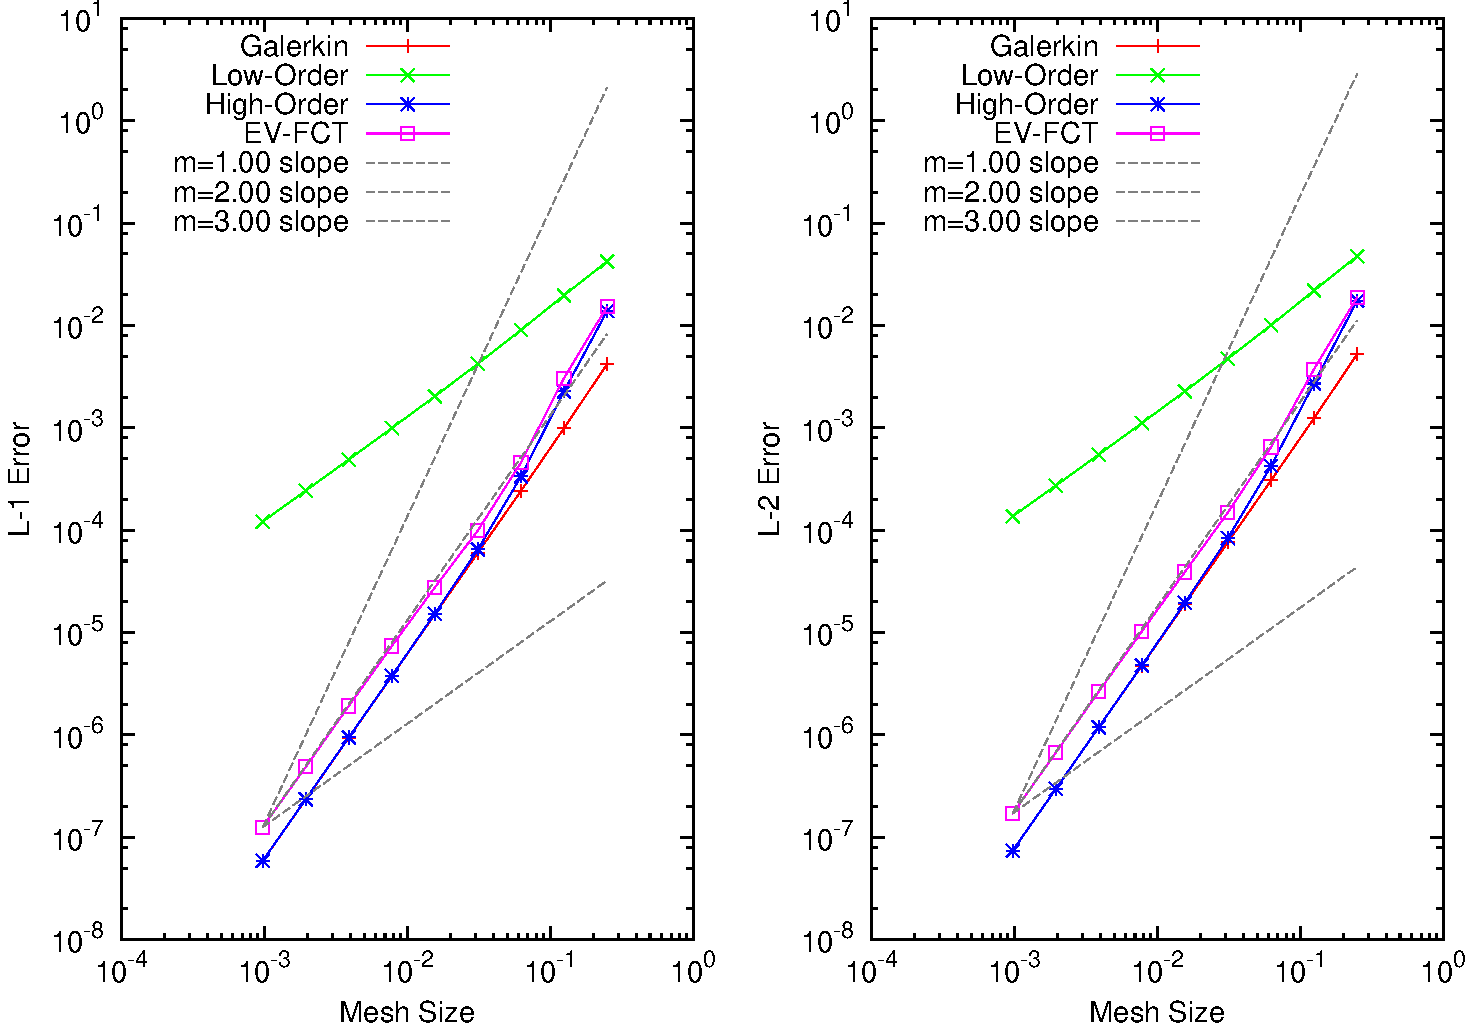
\includegraphics[height=0.8\textheight]{./figures/convergence_smooth_FE.pdf}
\end{center}

\end{frame}
%%%%%%%%%%%%%%%%%%%%%%%%%%%%%%%%%%%%%%%%%%%%%%%%%%%%%%%%%%%%%%%%%%%%%%%%%%%%%%%%%
\begin{frame}
\frametitle{1-D Non-smooth Problem Convergence Results (Using SSPRK33)}

\begin{center}
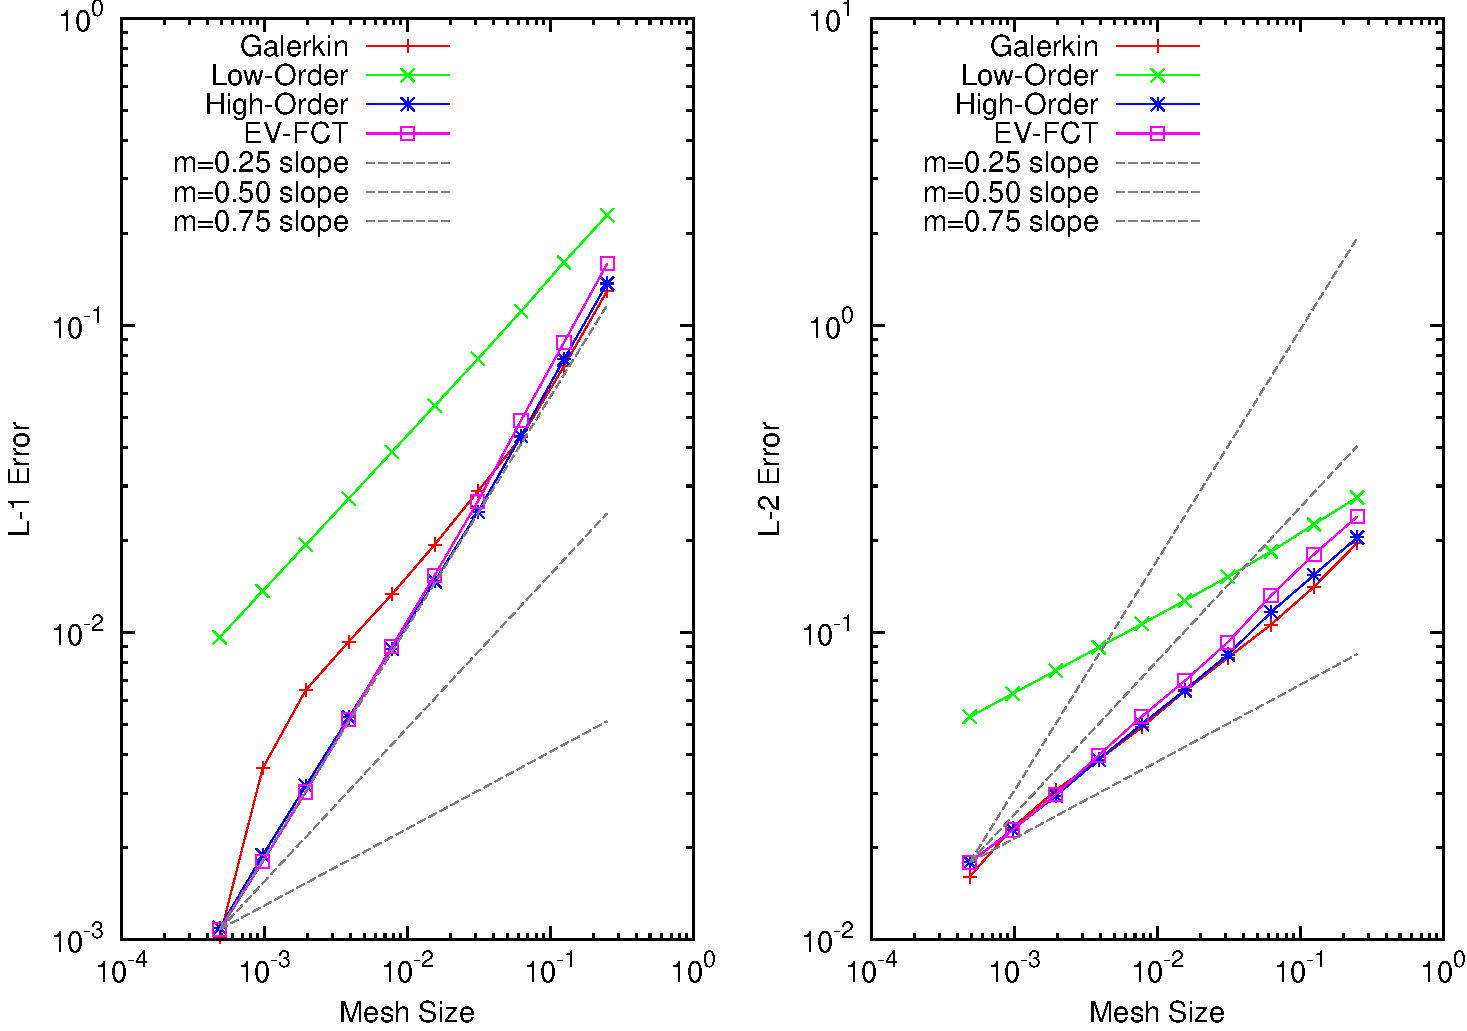
\includegraphics[height=0.8\textheight]{./figures/convergence_absorber_SSPRK33.pdf}
\end{center}

\end{frame}
%%%%%%%%%%%%%%%%%%%%%%%%%%%%%%%%%%%%%%%%%%%%%%%%%%%%%%%%%%%%%%%%%%%%%%%%%%%%%%%%%
\section{Shallow Water Equations Introduction}
\subsection{Introduction}
%%%%%%%%%%%%%%%%%%%%%%%%%%%%%%%%%%%%%%%%%%%%%%%%%%%%%%%%%%%%%%%%%%%%%%%%%%%%%%%%%
\begin{frame}
\frametitle{Shallow Water Equations (SWE) Introduction}

\begin{itemize}
  \item This research also considers the shallow water equations system:
    \begin{equation}
      \ppt{}\left[\begin{array}{c}\height\\\heightmomentum\end{array}\right]
        + \divergence\left[\begin{array}{c}\heightmomentum\\
          \heightmomentum\otimes\velocity + \half\gravity\height^2 I
          \end{array}\right]
        = \left[\begin{array}{c}0\\-\gravity\height\nabla\bathymetry\end{array}
    \right] \eqp
    \end{equation}
    \begin{itemize}
      \item $\height\xt \equiv \int\density\xt dz$ is referred to as ``height''.
      \item $\heightmomentum\xt \equiv \height\xt\velocity\xt$ is referred to
        as ``discharge''.
      \item $\gravity$ is the acceleration due to gravity.
      \item $\bathymetry(\x)$ is the bottom topography profile,
        or ``bathymetry''.
    \end{itemize}
  \item Obtained by depth-integrating Navier-Stokes equations with the
    assumption that the horizontal length scale is much greater than the
    vertical length scale
  \item Some important simulations include
    \begin{itemize}
      \item \textcolor{secondarycolorheavy}{dam break problems}: for example, what wave
        structures will develop in a dam-break accident?
      \item \textcolor{secondarycolorheavy}{wave/tsunami problems}: for example, what height
        of seawall is necessary to stop a wave of a certain height?
    \end{itemize}
\end{itemize}

\end{frame}
%%%%%%%%%%%%%%%%%%%%%%%%%%%%%%%%%%%%%%%%%%%%%%%%%%%%%%%%%%%%%%%%%%%%%%%%%%%%%%%%%
\subsection{Discretization}
%%%%%%%%%%%%%%%%%%%%%%%%%%%%%%%%%%%%%%%%%%%%%%%%%%%%%%%%%%%%%%%%%%%%%%%%%%%%%%%%%
\begin{frame}
\frametitle{Discretization}

\begin{itemize}
  \item A general system of conservation laws, with sources, is
    \begin{equation}
      \pd{\vectorsolution}{t} + \divergence\consfluxvector(\vectorsolution)
        = \conssource(\vectorsolution) \eqp
    \end{equation}
  \item After doing the following:
    \begin{itemize}
      \item Substituting the approximate solution
        $\approximatevectorsolution\xt =
          \sum_j \solutionvector_j(t) \testfunction_j(\x)$,
          where $\solutionvector_j(t)$ are vector-valued degrees of freedom,
      \item Interpolating the flux function at the nodes,
        $\consfluxvector(\approximatevectorsolution)\rightarrow
          \sum_j\consfluxinterpolant_j(t)\testfunction_j(\x)$,
      \item Testing with $\testfunction_i(\x)$, and
      \item Evaluating with forward Euler (FE),
    \end{itemize}
    the discrete system becomes
    \begin{equation}
      \sum_j\consistentmassentry
        \frac{\solutionvector_j^{n+1}-\solutionvector_j^n}{\dt}
        + \sum_j\gradiententry\cdot\consfluxinterpolant_j^n
        = \ssrhs_i^n \eqc
    \end{equation}
    \begin{equation}
      \gradiententry \equiv \int_{\support\ij}
        \testfunction_i(\x)\nabla\testfunction_j(\x) d\volume \eqc
      \quad
      \ssrhs_i(t) \equiv \int_{\support_i}
        \testfunction_i(\x)\conssource(\approximatevectorsolution)d\volume \eqp
    \end{equation}
\end{itemize}

\end{frame}
%%%%%%%%%%%%%%%%%%%%%%%%%%%%%%%%%%%%%%%%%%%%%%%%%%%%%%%%%%%%%%%%%%%%%%%%%%%%%%%%%
\section{Systems Methodology}
\subsection{Low-Order Scheme}
%%%%%%%%%%%%%%%%%%%%%%%%%%%%%%%%%%%%%%%%%%%%%%%%%%%%%%%%%%%%%%%%%%%%%%%%%%%%%%%%%
\begin{frame}
\frametitle{Invariant Domain}

\begin{itemize}
  \item For the \emph{systems} case, discrete maximum principles no longer apply;
    the concept of \hlorange{invariant domains} becomes the desired tool.
  \item The objective is to prove that the solution
    $\approximatevectorsolution^{n+1}\equiv\discreteprocess
      (\approximatevectorsolution^n)$ belongs to an invariant domain with
    respect to the discrete solution process $\discreteprocess$.
  \item First one assumes that the initial data belongs
    to a convex invariant admissible set: $\vectorsolution^0\in\invariantset$.
  \item Next one expresses $\discreteprocess(\approximatevectorsolution^n)$
    as a convex combination of states:
    $\sum_i\convexcoefficient_i\convexelement_i$, and proves the following:
    \begin{enumerate}
      \item $\sum_i \convexcoefficient_i = 1$
      \item $\convexcoefficient_i \geq 0 \quad \forall i$
      \item $\convexelement_i \in \invariantset \quad \forall i$
    \end{enumerate}
  \item Thus it is proven that
    $\discreteprocess(\approximatevectorsolution^n)\in\invariantset$ since
    $\invariantset$ is a convex set, and thus $\invariantset$ is an invariant
    domain for $\discreteprocess$.
\end{itemize}

\end{frame}
%%%%%%%%%%%%%%%%%%%%%%%%%%%%%%%%%%%%%%%%%%%%%%%%%%%%%%%%%%%%%%%%%%%%%%%%%%%%%%%%%
\begin{frame}
\frametitle{Low-Order Scheme}

\begin{itemize}
  \item The domain-invariant low-order scheme lumps the mass matrix and adds
    a low-order diffusion term:
    \begin{equation}
      \lumpedmassentry
        \frac{\solutionvector_i^{L,n+1}-\solutionvector_i^n}{\dt}
        + \sum_j\gradiententry\cdot\consfluxinterpolant_j^n
        + \sum_j\diffusionmatrixletter\ij^{L,n}\solutionvector_j^n
        = \ssrhs_i^n \eqc
    \end{equation}
  \item The following definition for the low-order diffusion matrix allows
    the domain-invariance property to be proven:
    \begin{equation}
      \diffusionmatrixletter^{L,n}\ij \equiv
        \max(\maxwavespeed\ij,\maxwavespeed\ji)
      \quad j\ne i \eqc \quad
      \diffusionmatrixletter^{L,n}_{i,i} \equiv
        -\sumjnoti\diffusionmatrixletter^{L,n}\ij
      \eqc
   \end{equation}
   where $\maxwavespeed\ij \equiv \maxwavespeed(
   \normalvector\ij,\solutionvector_i^n,\solutionvector_j^n)$
   is the maximum wave speed in the 1-D Riemann problem in the direction
   $\normalvector\ij \equiv \mathbf{\gradientmatrixletter}\ij /
   \ltwonorm{\mathbf{\gradientmatrixletter}\ij}$
   with left state $\solutionvector_i^n$ and right state $\solutionvector_j^n$.
\end{itemize}

\end{frame}
%%%%%%%%%%%%%%%%%%%%%%%%%%%%%%%%%%%%%%%%%%%%%%%%%%%%%%%%%%%%%%%%%%%%%%%%%%%%%%%%%
\subsection{High-Order Scheme}
%%%%%%%%%%%%%%%%%%%%%%%%%%%%%%%%%%%%%%%%%%%%%%%%%%%%%%%%%%%%%%%%%%%%%%%%%%%%%%%%%
\begin{frame}
\frametitle{High-Order Scheme}

\begin{itemize}
  \item The high-order scheme adds a high-order diffusion term:
    \begin{equation}
      \sum_j\consistentmassentry
        \frac{\solutionvector_j^{H,n+1}-\solutionvector_j^n}{\dt}
        + \sum_j\gradiententry\cdot\consfluxinterpolant_j^n
        + \sum_j\diffusionmatrixletter\ij^{H,n}\solutionvector_j^n
        = \ssrhs_i^n \eqc
    \end{equation}
  \item The high-order diffusion matrix is proportional to an entropy diffusion matrix
    and uses the low-order diffusion matrix as an upper bound:
    \begin{equation}
      \diffusionmatrixletter^{H,n}\ij \equiv \min(
        \diffusionmatrixletter^{\entropy,n}\ij,\diffusionmatrixletter^{L,n}\ij) \eqc
    \end{equation}
    where the entropy diffusion matrix is proportional to an entropy residual and
    entropy jump:
    \begin{equation}
      \diffusionmatrixletter^{\entropy,n}\ij \equiv
        \frac{\entropyresidualcoef\entropyresidual\ij^n
          + \entropyjumpcoef\entropyjump\ij^n}{\entropynormalization\ij^n} \eqp
    \end{equation}
\end{itemize}

\end{frame}
%%%%%%%%%%%%%%%%%%%%%%%%%%%%%%%%%%%%%%%%%%%%%%%%%%%%%%%%%%%%%%%%%%%%%%%%%%%%%%%%%
\begin{frame}
\frametitle{Entropy for the Shallow Water Equations}

\begin{itemize}
  \item For the SWE, the entropy is chosen to be the sum of kinetic and
    potential energy terms:
    \begin{equation}
      \entropy(\vectorsolution,\bathymetry)
        = \half\frac{\heightmomentum\cdot\heightmomentum}{\height}
          + \half\gravity\height\pr{\height+\bathymetry}
      \eqp
    \end{equation}
  \item The entropy flux is
    \begin{equation}
      \mathbf{\consfluxletter}^\entropy(\vectorsolution,\bathymetry)
        = \gravity(\height + \bathymetry)\heightmomentum
        + \half\frac{\pr{\heightmomentum\cdot\heightmomentum}\heightmomentum} 
        {\height^2}
      \eqp
    \end{equation}
  \item The entropy residual is
    \begin{equation}
      \entropyresidual(\vectorsolution^\timeindex, \vectorsolution^{\timeindex-1})
        \equiv \frac{\entropy(\vectorsolution^\timeindex)
        - \entropy(\vectorsolution^{\timeindex-1})}{\timestepsize^{\timeindex-1}}
        + \divergence\mathbf{\consfluxletter}^\entropy(\vectorsolution^\timeindex,
          \bathymetry)
      \eqp
    \end{equation}
\end{itemize}

\end{frame}
%%%%%%%%%%%%%%%%%%%%%%%%%%%%%%%%%%%%%%%%%%%%%%%%%%%%%%%%%%%%%%%%%%%%%%%%%%%%%%%%%
\subsection{FCT Scheme}
%%%%%%%%%%%%%%%%%%%%%%%%%%%%%%%%%%%%%%%%%%%%%%%%%%%%%%%%%%%%%%%%%%%%%%%%%%%%%%%%%
\begin{frame}
\frametitle{FCT Antidiffusive Flux Definition}

\begin{itemize}
  \item The antidiffusive fluxes $\correctionfluxvector_i$ are defined such that
    \begin{equation}
      \lumpedmassentry
        \frac{\solutionvector_i^{H,n+1}-\solutionvector_i^n}{\dt}
        + \sum_j\gradiententry\cdot\consfluxinterpolant_j^n
        + \sum_j\diffusionmatrixletter\ij^{L,n}\solutionvector_j^n
        = \ssrhs_i^n + \correctionfluxvector_i\eqc
    \end{equation}
   \item Subtracting the high-order scheme equation from this gives the
      definition of $\correctionfluxvector$:
      \begin{equation}
        \correctionfluxvector_i \equiv
          \lumpedmassentry
            \frac{\solutionvector_i^{H}-\solutionvector_i^n}{\dt}
          -\sum_j\consistentmassentry
            \frac{\solutionvector_j^{H}-\solutionvector_j^n}{\dt}
          +\sum_j(\diffusionmatrixletter\ij^{L,n}-\diffusionmatrixletter\ij^{H,n})
            \solutionvector_j^n
      \end{equation}
   \item Decomposing $\correctionfluxvector$ into internodal fluxes
      $\correctionfluxmatrix\ij$ such that $\sum_j \correctionfluxmatrix\ij =
      \correctionfluxvector_i$,
      \begin{equation}
        \correctionfluxmatrix\ij = -M\ij^C\pr{
            \frac{\solutionvector_j^{H}-\solutionvector_j^n}{\dt}
            -\frac{\solutionvector_i^{H}-\solutionvector_i^n}{\dt}
          }
          + (D\ij^{L,n}-D\ij^{H,n})(\solutionvector_j^n-\solutionvector_i^n) \eqp
      \end{equation}
\end{itemize}

\end{frame}
%%%%%%%%%%%%%%%%%%%%%%%%%%%%%%%%%%%%%%%%%%%%%%%%%%%%%%%%%%%%%%%%%%%%%%%%%%%%%%%%%
\begin{frame}
\frametitle{Limiting Coefficients}

\begin{itemize}
  \item Bounds to impose on solution are unclear:
    \begin{itemize}
      \item For scalar case, a DMP was used, but no DMP exists for systems.
      \item The invariant domain property is not useful here
        because the invariant domain is not actually known.
    \end{itemize}
  \item Choose to impose LED constraint for each component:
    \begin{equation}
      \solutionletter_{\min,i}^{\componentindex,n}
        \leq \solutionletter_i^{\componentindex,n+1}
        \leq \solutionletter_{\max,i}^{\componentindex,n}
      \quad \forall\componentindex \eqp
    \end{equation}
  \item The FCT scheme is
    \begin{equation}
      \lumpedmassentry
        \frac{\solutionvector_i^{n+1}-\solutionvector_i^n}{\dt}
        + \sum_j\gradiententry\cdot\consfluxinterpolant_j^n
        + \sum_j\diffusionmatrixletter\ij^{L,n}\solutionvector_j^n
        = \ssrhs_i^n + \sum_j\limitermatrix\ij\odot\correctionfluxmatrix\ij \eqp
    \end{equation}
\end{itemize}

\end{frame}
%%%%%%%%%%%%%%%%%%%%%%%%%%%%%%%%%%%%%%%%%%%%%%%%%%%%%%%%%%%%%%%%%%%%%%%%%%%%%%%%%
\begin{frame}
\frametitle{Limiting Coefficients (Cont.)}

\begin{itemize}
  \item Define antidiffusive flux bounds $\mathbf{\limitedfluxbound}_i^\pm$ such that
    \begin{equation}
      \mathbf{\limitedfluxbound}^-_i \leq
        \sum\limits_j \limitermatrix\ij\odot\correctionfluxmatrix\ij \leq
        \mathbf{\limitedfluxbound}^+_i
      \quad\Rightarrow\quad
      \mathbf{\DMPbound}_i^- \leq
        \solutionvector_i^{n+1} \leq
        \mathbf{\DMPbound}_i^+ \quad \forall i \eqp
    \end{equation}
  \item Performing some algebra gives the definition
    \begin{equation}
      \mathbf{\limitedfluxbound}_i^\pm \equiv
        \lumpedmassentry\frac{\mathbf{\DMPbound}_i^\pm-\solutionvector_i^n}{\dt}
        + \sum_j\gradiententry\cdot\consfluxinterpolant_j^n
        + \sum_j\diffusionmatrixletter\ij^{L,n}\solutionvector_j^n
        - \ssrhs_i^n \eqp
    \end{equation}
  \item As in the scalar case, negative and positive antidiffusive flux
    sums are required in the limiting coefficient definitions:
    \begin{equation}
      \correctionfluxletter_i^{\componentindex,-} \equiv
        \sum\limits_{j:\correctionfluxij^\componentindex<0}
        \correctionfluxij^\componentindex \eqc \qquad
      \correctionfluxletter_i^{\componentindex,+} \equiv
        \sum\limits_{j:\correctionfluxij^\componentindex>0}
        \correctionfluxij^\componentindex \eqp
    \end{equation}
\end{itemize}

\end{frame}
%%%%%%%%%%%%%%%%%%%%%%%%%%%%%%%%%%%%%%%%%%%%%%%%%%%%%%%%%%%%%%%%%%%%%%%%%%%%%%%%%
\begin{frame}
\frametitle{Limiting Coefficients (Cont.)}

\begin{itemize}
  \item The limiting coefficients are first computed just as in the scalar case:
    \begin{equation}
      \limiterletter_i^{\componentindex,\pm} \equiv\left\{
        \begin{array}{l l}
          1 & \correctionfluxletter_i^{\componentindex,\pm} = 0\\
          \min\left(1,\frac{Q_i^{\componentindex,\pm}}
            {\correctionfluxletter_i^{\componentindex,\pm}}\right) &
          \correctionfluxletter_i^{\componentindex,\pm} \ne 0
        \end{array}
      \right. \eqp
    \end{equation}
    \begin{equation}
      \limiterletter\ij^\componentindex \equiv\left\{
        \begin{array}{l l}
          \min(L_i^{\componentindex,+},L_j^{\componentindex,-}) &
            \correctionfluxij^\componentindex \geq 0\\
          \min(L_i^{\componentindex,-},L_j^{\componentindex,+}) &
            \correctionfluxij^\componentindex < 0
        \end{array}
      \right. \eqp
    \end{equation}
  \item However, there is a caveat: limiting coefficients may require
    \hlorange{synchronization}, e.g.,
    \begin{equation}
      \limiterletter\ij^\componentindex \mapsfrom
        \min\limits_k\limiterletter\ij^k \quad \forall\componentindex \eqp
    \end{equation}
  \item Otherwise, antidiffusive fluxes in one component can violate the
    conditions of another component.
\end{itemize}

\end{frame}
%%%%%%%%%%%%%%%%%%%%%%%%%%%%%%%%%%%%%%%%%%%%%%%%%%%%%%%%%%%%%%%%%%%%%%%%%%%%%%%%%
\section{Shallow Water Equations Results}
%%%%%%%%%%%%%%%%%%%%%%%%%%%%%%%%%%%%%%%%%%%%%%%%%%%%%%%%%%%%%%%%%%%%%%%%%%%%%%%%%
\begin{frame}
\frametitle{Preliminary Results}
\framesubtitle{Height in Dam Break Problem}

\begin{center}
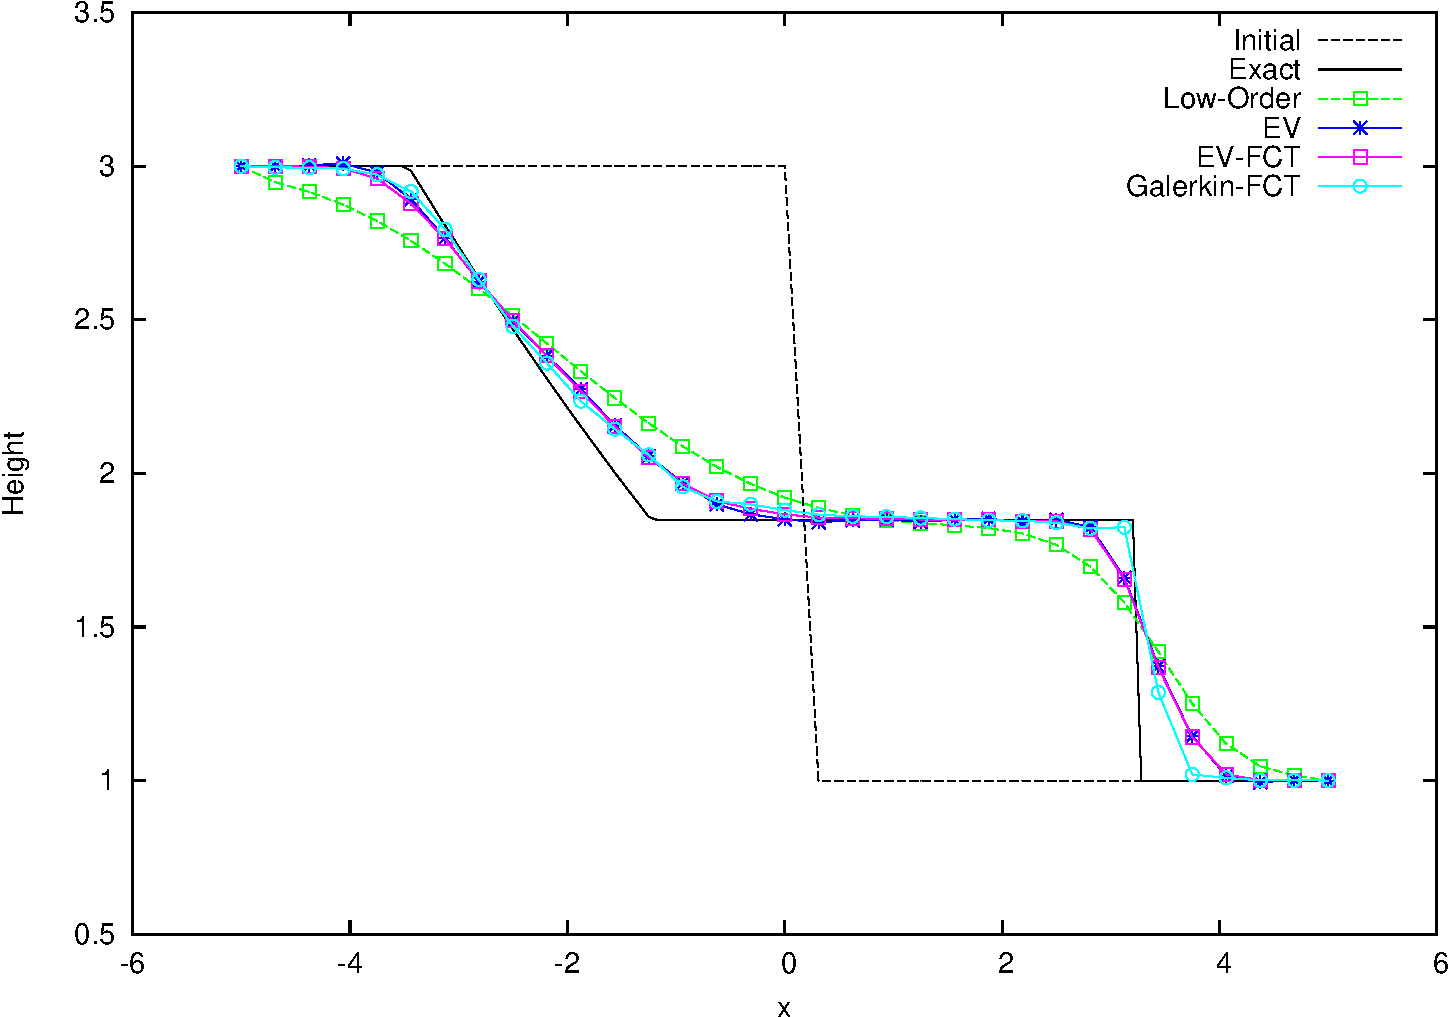
\includegraphics[height=0.8\textheight]{./figures/height_FE.pdf}
\end{center}

\end{frame}
%%%%%%%%%%%%%%%%%%%%%%%%%%%%%%%%%%%%%%%%%%%%%%%%%%%%%%%%%%%%%%%%%%%%%%%%%%%%%%%%%
\begin{frame}
\frametitle{Preliminary Results}
\framesubtitle{Discharge in Dam Break Problem}

\begin{center}
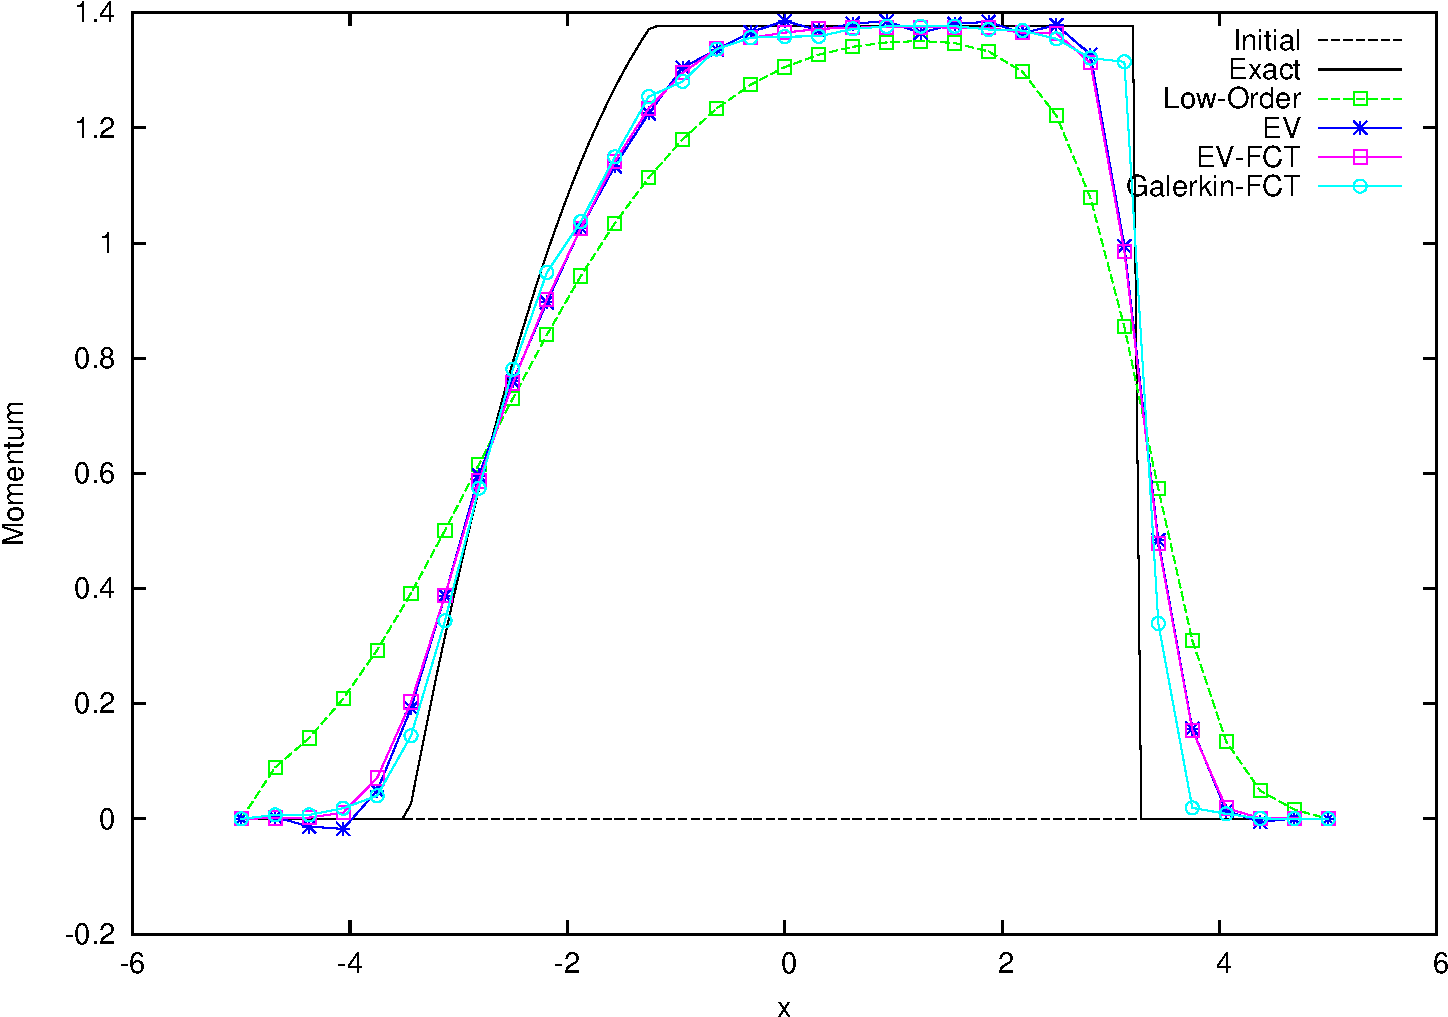
\includegraphics[height=0.8\textheight]{./figures/momentum_FE.pdf}
\end{center}

\end{frame}
%%%%%%%%%%%%%%%%%%%%%%%%%%%%%%%%%%%%%%%%%%%%%%%%%%%%%%%%%%%%%%%%%%%%%%%%%%%%%%%%%
\section{Conclusions}
%%%%%%%%%%%%%%%%%%%%%%%%%%%%%%%%%%%%%%%%%%%%%%%%%%%%%%%%%%%%%%%%%%%%%%%%%%%%%%%%%
\begin{frame}
\frametitle{Progress}

\begin{itemize}
  \item Scalar Conservation Laws:
    \begin{itemize}
      \item[\checked] Low-order, DMP-satisfying, positivity-preserving scheme
      \item[\checked] High-order, entropy-based scheme
      \item[\checked] High-order, DMP-satisfying, positivity-preserving FCT scheme
    \end{itemize}
 \item Systems of Conservation Laws / Shallow Water Equations (SWE):
   \begin{itemize}
     \item[\checked] Low-order, domain-invariant, positivity-preserving scheme
       for SWE with \emph{flat} bottom topography
     \item[\unchecked] Low-order, domain-invariant, positivity-preserving scheme
       for SWE with \emph{non-flat} bottom topography
     \item[\checked] High-order, entropy-based scheme
     \item[\unchecked] High-order, LED, positivity-preserving FCT scheme
   \end{itemize}
\end{itemize}

\end{frame}
%%%%%%%%%%%%%%%%%%%%%%%%%%%%%%%%%%%%%%%%%%%%%%%%%%%%%%%%%%%%%%%%%%%%%%%%%%%%%%%%%
\begin{frame}
\frametitle{Conclusions}

\begin{itemize}
  \item The scalar FCT scheme developed is
    \begin{itemize}
      \item Positivity-preserving
      \item Discrete-maximum-principle preserving
      \item Not guaranteed monotone, but works well in practice
      \item Entropy-inequality-enforcing
      \item 2nd-order-accurate for smooth problems
      \item Valid in an arbitrary number of dimensions
      \item Valid for general meshes
    \end{itemize}
  \item The shallow water equations FCT scheme developed is
    \begin{itemize}
      \item Positivity-preserving
      \item Not guaranteed monotone, but works well in practice
      \item Entropy-inequality-enforcing
      \item 2nd-order-accurate for smooth problems
      \item Valid in an arbitrary number of dimensions (in general - the SWE
        do not apply in 3-D of course)
      \item Valid for general meshes
    \end{itemize}
\end{itemize}

\end{frame}
%%%%%%%%%%%%%%%%%%%%%%%%%%%%%%%%%%%%%%%%%%%%%%%%%%%%%%%%%%%%%%%%%%%%%%%%%%%%%%%%
\begin{frame}
\frametitle{Acknowledgments}

\begin{itemize}
   \item Dr. Jean Ragusa
   \item Dr. Jean-Luc Guermond
   \item Dr. Marco Delchini
   \item Dr. Dmitri Kuzmin
\end{itemize}
\begin{itemize}
   \item This material is based upon work supported under an Integrated University
      Program Graduate Fellowship.
\end{itemize}

\begin{center}
   
\includegraphics[width=0.4\textwidth]{./figures/NEUP_Final_Logo_Version-09.jpg}
\end{center}
\end{frame}
%%%%%%%%%%%%%%%%%%%%%%%%%%%%%%%%%%%%%%%%%%%%%%%%%%%%%%%%%%%%%%%%%%%%%%%%%%%%%%%%%
\end{document}
